% =============================================================================
%  Diplomado en Data Science Aplicada con Python para la Toma de Decisiones
%  Clase 21: PCA + K-Means --- Reduccion de Dimension y Segmentacion
%  Arca Continental Ecuador | UDLA
%
%  Compilar: pdflatex -shell-escape presentacion.tex (x2 para refs)
% =============================================================================
\documentclass[aspectratio=169, 11pt]{beamer}

\usepackage[T1]{fontenc}
\usepackage[utf8]{inputenc}
\usepackage[spanish,es-noshorthands]{babel}
\usepackage{FiraSans}
\usepackage{FiraMono}
\renewcommand{\familydefault}{\sfdefault}
\usepackage{graphicx}
\usepackage{tikz}
\usetikzlibrary{arrows.meta, positioning, shapes.geometric, shapes.misc,
  calc, fit, decorations.pathreplacing, backgrounds}
\usepackage{fontawesome5}
\usepackage{minted}
\usepackage{tcolorbox}
\tcbuselibrary{minted, skins, breakable}
\usepackage{booktabs}
\usepackage{colortbl}
\usepackage{multicol}
\usepackage{hyperref}
\usepackage{calc}
\usepackage{amsmath}

\definecolor{arcaRed}{HTML}{C82B40}
\definecolor{arcaDark}{HTML}{6B1525}
\definecolor{udlaCrimson}{HTML}{A31545}
\definecolor{arcaGray}{HTML}{F5F5F5}
\definecolor{arcaLightGray}{HTML}{EBEBEB}
\definecolor{textDark}{HTML}{2D2D2D}
\definecolor{textMuted}{HTML}{6B7280}
\definecolor{codeGreen}{HTML}{16A34A}
\definecolor{codeBlue}{HTML}{2563EB}
\definecolor{codeOrange}{HTML}{EA580C}
\definecolor{codePurple}{HTML}{7C3AED}

\usetheme{default}
\usecolortheme{default}
\setbeamertemplate{navigation symbols}{}
\setbeamertemplate{footline}{}
\setbeamertemplate{headline}{}
\setbeamercolor{normal text}{fg=textDark}
\setbeamercolor{frametitle}{fg=arcaRed, bg=white}
\setbeamercolor{title}{fg=white}
\setbeamercolor{subtitle}{fg=white!85}
\setbeamercolor{author}{fg=white!80}
\setbeamercolor{date}{fg=white!70}
\setbeamercolor{item}{fg=arcaRed}
\setbeamercolor{subitem}{fg=arcaDark}
\setbeamercolor{block title}{fg=white, bg=arcaRed}
\setbeamercolor{block body}{fg=textDark, bg=arcaGray}
\setbeamercolor{block title alerted}{fg=white, bg=codeOrange}
\setbeamercolor{block body alerted}{fg=textDark, bg=arcaGray}
\setbeamercolor{block title example}{fg=white, bg=codeGreen}
\setbeamercolor{block body example}{fg=textDark, bg=arcaGray}
\setbeamercolor{section in toc}{fg=arcaDark}
\setbeamerfont{frametitle}{size=\Large, series=\bfseries}
\setbeamerfont{title}{size=\huge, series=\bfseries}
\setbeamerfont{subtitle}{size=\large}
\setbeamerfont{author}{size=\normalsize}
\setbeamerfont{date}{size=\small}
\setbeamerfont{block title}{size=\normalsize, series=\bfseries}
\setbeamerfont{footnote}{size=\tiny}
\setbeamertemplate{itemize item}{\scriptsize\raise1.5pt\hbox{\color{arcaRed}$\blacktriangleright$}}
\setbeamertemplate{itemize subitem}{\scriptsize\raise1pt\hbox{\color{arcaDark}$\bullet$}}
\setbeamertemplate{enumerate items}[default]
\setbeamercolor{enumerate item}{fg=arcaRed}

\setbeamertemplate{headline}{%
  \begin{tikzpicture}[remember picture, overlay]
    \fill[arcaDark] (current page.north west) rectangle
      ([yshift=-0.7cm]current page.north east);
    \node[anchor=west, inner sep=0pt] at
      ([xshift=0.6cm, yshift=-0.35cm]current page.north west)
      {
\includegraphics[height=0.45cm]{../logo_udla_white.png}};
    \node[anchor=east, inner sep=0pt] at
      ([xshift=-0.6cm, yshift=-0.35cm]current page.north east)
      {
\includegraphics[height=0.45cm]{../ArcaContinental_white.png}};
  \end{tikzpicture}%
  \vspace{0.7cm}%
}

\setbeamertemplate{footline}{%
  \begin{tikzpicture}[remember picture, overlay]
    \node[anchor=south east, font=\scriptsize\bfseries\color{arcaRed}] at
      ([xshift=-0.5cm, yshift=0.15cm]current page.south east)
      {\insertframenumber};
  \end{tikzpicture}%
  \vspace{0.3cm}%
}

\setbeamertemplate{frametitle}{%
  \vspace{0.25cm}%
  \usebeamerfont{frametitle}\usebeamercolor[fg]{frametitle}\insertframetitle%
  \par\vspace{2pt}%
  \begin{tikzpicture}
    \fill[arcaRed] (0,0) rectangle (3cm, 1.5pt);
    \fill[arcaLightGray] (3cm,0) rectangle (\textwidth, 0.5pt);
  \end{tikzpicture}%
  \vspace{0.1cm}%
}

\newtcblisting{pyblock}[1][]{%
  listing engine=minted, minted language=python, minted style=friendly,
  minted options={fontsize=\small, linenos=false, breaklines=true, python3=true},
  colback=arcaGray, colframe=arcaRed, left=4pt, right=4pt, top=4pt, bottom=4pt,
  boxrule=0pt, leftrule=3pt, arc=2pt, listing only, #1}

\newtcblisting{outputblock}[1][]{%
  listing engine=minted, minted language=text, minted style=bw,
  minted options={fontsize=\small, breaklines=true},
  colback=white, colframe=arcaLightGray, left=4pt, right=4pt, top=4pt, bottom=4pt,
  boxrule=0.5pt, arc=2pt, listing only,
  title={\small\faTerminal\hspace{6pt}Output}, coltitle=textMuted,
  fonttitle=\small\ttfamily, colbacktitle=white, #1}

\newcommand{\sectionframe}[2]{%
  \begingroup
  \setbeamertemplate{headline}{}%
  \setbeamertemplate{footline}{}%
  \begin{frame}[plain, noframenumbering]
    \begin{tikzpicture}[remember picture, overlay]
      \fill[arcaRed] (current page.south west) rectangle (current page.north east);
      \node[anchor=center, text=white, font=\Huge\bfseries, text width=12cm,
            align=center] at ([yshift=0.5cm]current page.center) {#1};
      \node[anchor=center, text=white!80, font=\large, text width=10cm,
            align=center] at ([yshift=-0.8cm]current page.center) {#2};
    \end{tikzpicture}
  \end{frame}
  \endgroup
}

\title{Diplomado en Data Science Aplicada\\con Python para la Toma de Decisiones}
\subtitle{Clase 21: PCA + K-Means --- Comprimir y Segmentar}
\author{Carlos Enrique Mosquera Trujillo}
\date{4 de Mayo, 2026}

\begin{document}

% ── PORTADA ──────────────────────────────────────────────────────────────────
{
\setbeamertemplate{headline}{}
\setbeamertemplate{footline}{}
\begin{frame}[plain, noframenumbering]
  \begin{tikzpicture}[remember picture, overlay]
    \fill[arcaDark] (current page.south west) rectangle (current page.north east);
    \fill[arcaRed] ([yshift=-3.5cm]current page.north west) rectangle
      ([yshift=-4.2cm]current page.north east);
    \node[anchor=west, inner sep=0pt] at
      ([xshift=1cm, yshift=-1.5cm]current page.north west)
      {
\includegraphics[height=1cm]{../logo_udla_white.png}};
    \node[anchor=east, inner sep=0pt] at
      ([xshift=-1cm, yshift=-1.5cm]current page.north east)
      {
\includegraphics[height=1cm]{../ArcaContinental_white.png}};
  \end{tikzpicture}
  \vspace{2.5cm}
  \begin{center}
    {\usebeamerfont{title}\usebeamercolor[fg]{title}\inserttitle\par}
    \vspace{0.4cm}
    {\usebeamerfont{subtitle}\usebeamercolor[fg]{subtitle}\insertsubtitle\par}
    \vspace{0.6cm}
    {\usebeamerfont{author}\usebeamercolor[fg]{author}\insertauthor\par}
    \vspace{0.15cm}
    {\usebeamerfont{date}\usebeamercolor[fg]{date}\insertdate\par}
  \end{center}
\end{frame}
}

% ── MÓDULO 4 ─────────────────────────────────────────────────────────────────
{
\setbeamertemplate{headline}{}
\setbeamertemplate{footline}{}
\begin{frame}[plain, noframenumbering]
  \begin{tikzpicture}[remember picture, overlay]
    \fill[arcaDark] (current page.south west) rectangle (current page.north east);
    \node[anchor=center, text=white, font=\Large\bfseries, text width=12cm,
          align=center] at ([yshift=1cm]current page.center)
      {M\'odulo 4 --- clase 8};
    \node[anchor=center, text=white!90, font=\huge\bfseries, text width=12cm,
          align=center] at ([yshift=-0.3cm]current page.center)
      {Machine Learning};
  \end{tikzpicture}
\end{frame}
}

% ── ROADMAP ─────────────────────────────────────────────────────────────────
\begin{frame}[shrink=22]{Hoja de Ruta de Hoy}
  \vspace{-4pt}
  \begin{center}
  \begin{tikzpicture}[
    node distance=0.35cm,
    roadstep/.style={rectangle, rounded corners=4pt, draw=arcaRed, fill=arcaRed!8,
                 minimum width=11cm, minimum height=0.65cm,
                 font=\footnotesize\bfseries\color{arcaDark}, align=left,
                 text width=10cm, inner sep=6pt},
    num/.style={circle, fill=arcaRed, text=white, font=\scriptsize\bfseries,
                minimum size=0.5cm, inner sep=0pt},
  ]
    \node[roadstep] (s0) {\hspace{0.8cm}El problema: demasiadas variables para visualizar};
    \node[roadstep, below=of s0] (s1) {\hspace{0.8cm}PCA: comprimir dimensiones sin perder informaci\'on};
    \node[roadstep, below=of s1] (s2) {\hspace{0.8cm}Scree plot: cu\'antos componentes conservar};
    \node[roadstep, below=of s2] (s3) {\hspace{0.8cm}Interpretar los componentes: loadings};
    \node[roadstep, below=of s3] (s4) {\hspace{0.8cm}Pipeline: PCA + K-Means (comprimir, luego segmentar)};
    \node[roadstep, below=of s4] (s5) {\hspace{0.8cm}Aplicaci\'on: World Happiness Report (151 pa\'ises, 7 variables)};
    \node[roadstep, below=of s5] (s6) {\hspace{0.8cm}Interpretaci\'on: qu\'e define la felicidad de un pa\'is};

    \node[num] at ([xshift=0.45cm]s0.west) {1};
    \node[num] at ([xshift=0.45cm]s1.west) {2};
    \node[num] at ([xshift=0.45cm]s2.west) {3};
    \node[num] at ([xshift=0.45cm]s3.west) {4};
    \node[num] at ([xshift=0.45cm]s4.west) {5};
    \node[num] at ([xshift=0.45cm]s5.west) {6};
    \node[num] at ([xshift=0.45cm]s6.west) {7};
  \end{tikzpicture}
  \end{center}
\end{frame}

% =============================================================================
%  BLOQUE A: LA MALDICI\'ON DE LA DIMENSIONALIDAD
% =============================================================================
\sectionframe{La Maldici\'on de la Dimensionalidad}{?`Por qu\'e muchas variables son un problema?}

\begin{frame}{Muchas Variables Parecen Buenas\ldots Pero No Siempre}
  \vspace{-4pt}
  {\footnotesize\color{arcaDark}\bfseries
    La intuici\'on dice: ``m\'as datos = mejor''. Pero con las
    \textbf{dimensiones} (variables) pasa algo contraintuitivo.}

  \vspace{6pt}
  {\footnotesize
  \begin{itemize}\setlength{\itemsep}{5pt}
    \item[{\color{arcaRed}\scriptsize\faArrowRight}]
      \textbf{Las distancias pierden significado:} en dimensiones altas,
      \textbf{todos los puntos est\'an casi a la misma distancia} entre s\'i.
      K-Means depende de distancias $\to$ si todas son iguales, no puede
      distinguir clusters.
    \item[{\color{arcaRed}\scriptsize\faArrowRight}]
      \textbf{Los modelos necesitan m\'as datos:} con 2 variables, 100
      observaciones cubren el espacio. Con 100 variables, 100 observaciones
      son un desierto --- el espacio es enorme y los datos son escasos.
    \item[{\color{arcaRed}\scriptsize\faArrowRight}]
      \textbf{Overfitting:} m\'as variables = m\'as oportunidades de
      encontrar correlaciones \textit{falsas} que solo existen en train.
    \item[{\color{arcaRed}\scriptsize\faArrowRight}]
      \textbf{Visualizaci\'on:} imposible ver m\'as de 3 dimensiones.
  \end{itemize}
  }
\end{frame}

\begin{frame}[shrink=15]{Las Distancias Se Vuelven In\'utiles}
  \vspace{-4pt}
  \begin{center}
    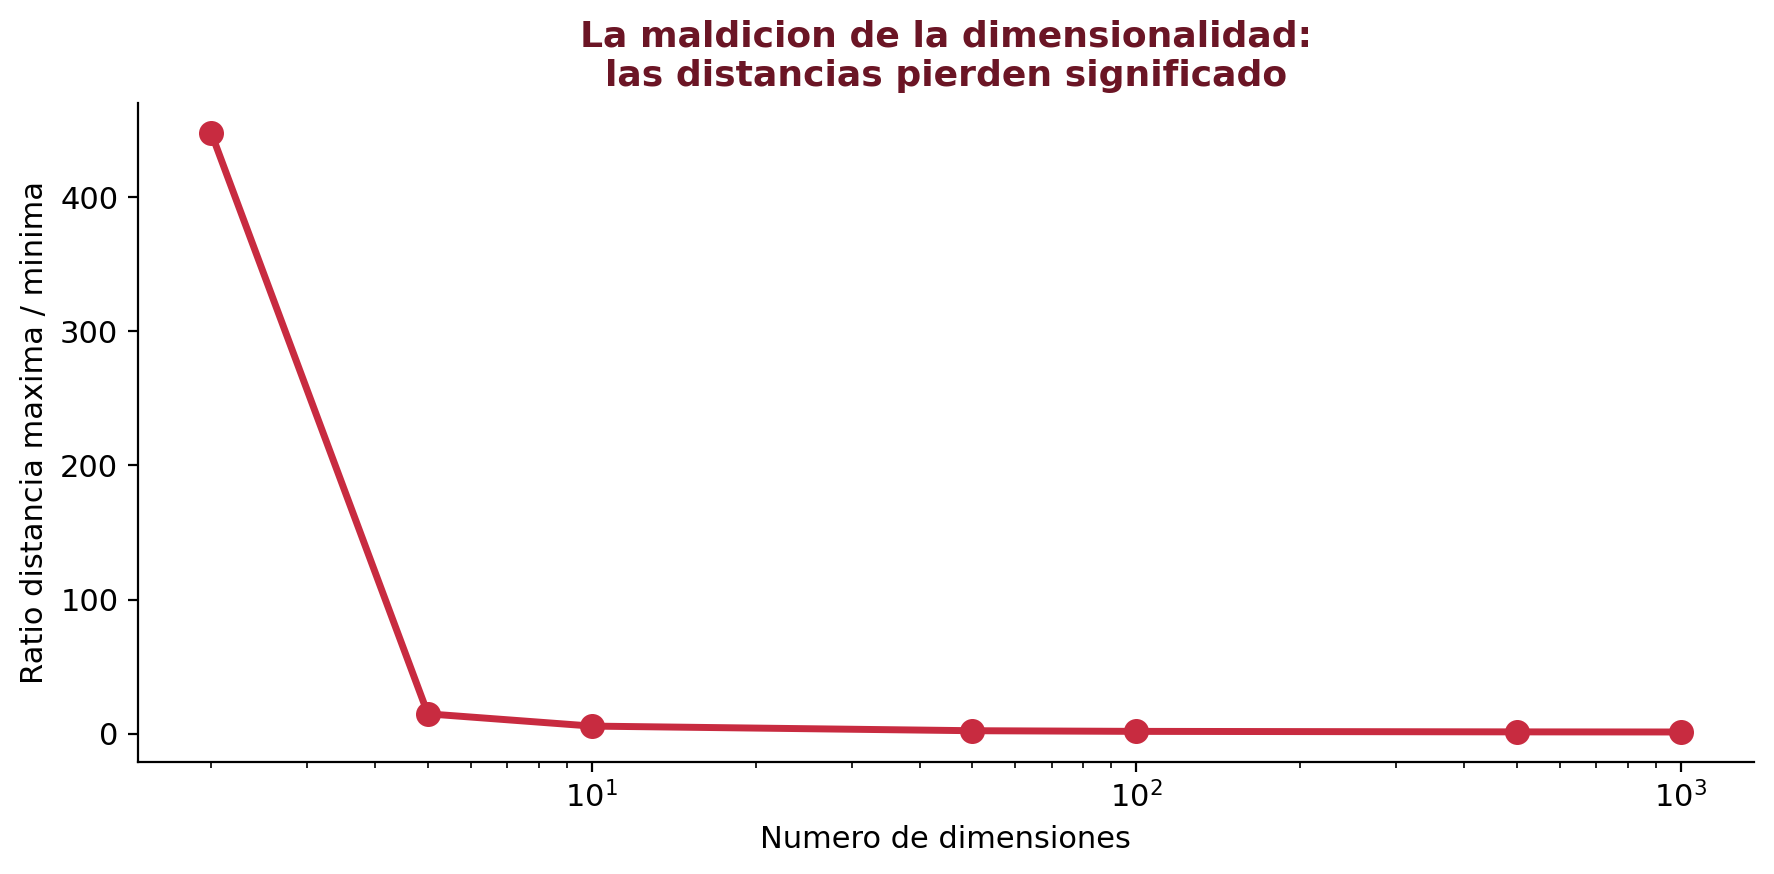
\includegraphics[width=0.78\textwidth]{fig_maldicion.png}
  \end{center}

  \vspace{-2pt}
  {\scriptsize\color{textMuted}
    \faLightbulb\hspace{4pt} Con 2 dimensiones, el punto m\'as lejano
    est\'a \textbf{mucho m\'as lejos} que el m\'as cercano (ratio alto).
    Con 1000 dimensiones, la diferencia entre el m\'as lejano y el m\'as
    cercano es m\'inima. Todos los puntos est\'an ``igual de lejos''.
    \textbf{Las distancias dejan de discriminar.}}
\end{frame}

\begin{frame}{?`Cu\'ando Se Vuelve un Problema?}
  \vspace{-4pt}
  {\footnotesize\color{arcaDark}\bfseries
    No siempre tener muchas variables es malo. Depende de la relaci\'on
    entre dimensiones y observaciones:}

  \vspace{6pt}
  {\scriptsize
  \begin{tabular}{@{}p{3.5cm}p{4.5cm}p{4.5cm}@{}}
    \toprule
    \textbf{Situaci\'on} & \textbf{Problema} & \textbf{Soluci\'on} \\
    \midrule
    Muchas variables correlacionadas & Redundancia: 5 variables dicen lo mismo. & PCA: comprimir en pocas componentes. \\
    M\'as variables que filas ($p > n$) & El modelo memoriza, no generaliza. & Reducci\'on de dimensi\'on o selecci\'on de variables. \\
    Variables ruidosas & Confunden al modelo sin aportar info. & PCA descarta las componentes de baja varianza (ruido). \\
    Visualizaci\'on imposible & No podemos hacer un scatter de 50 variables. & PCA a 2--3 componentes. \\
    \bottomrule
  \end{tabular}
  }

  \vspace{6pt}
  \begin{tcolorbox}[colback=codeGreen!8, colframe=codeGreen, boxrule=0.5pt, arc=2pt,
    left=6pt, right=6pt, top=4pt, bottom=4pt]
    {\scriptsize\color{arcaDark}
    \faCheckCircle\hspace{4pt}\textbf{Regla pr\'actica:} si tienes menos
    de 10 variables num\'ericas y suficientes datos, PCA no es urgente.
    Si tienes 50+, o variables muy correlacionadas, o quieres visualizar,
    PCA es tu herramienta.}
  \end{tcolorbox}
\end{frame}

% =============================================================================
%  BLOQUE A2: EL PROBLEMA APLICADO
% =============================================================================
\sectionframe{El Caso de Hoy}{World Happiness Report}

\begin{frame}{7 Variables = 21 Scatters Posibles}
  \vspace{-4pt}
  {\footnotesize\color{arcaDark}\bfseries
    El World Happiness Report mide 7 indicadores por pa\'is:
    econom\'ia, familia, salud, libertad, generosidad, corrupci\'on y
    satisfacci\'on laboral. ?`C\'omo los visualizamos todos a la vez?}

  \vspace{6pt}
  {\footnotesize
  \begin{itemize}\setlength{\itemsep}{5pt}
    \item[{\color{arcaRed}\scriptsize\faArrowRight}]
      Con 2 variables hacemos un scatter. Con 3, un scatter 3D.
    \item[{\color{arcaRed}\scriptsize\faArrowRight}]
      Con 7 variables tendr\'iamos que hacer $\binom{7}{2} = 21$
      scatters diferentes para ver todas las combinaciones.
    \item[{\color{arcaRed}\scriptsize\faArrowRight}]
      Y cada scatter solo muestra \textbf{dos} de las siete
      dimensiones --- perdemos el 71\% de la informaci\'on.
  \end{itemize}
  }

  \vspace{6pt}
  \begin{tcolorbox}[colback=arcaGray, colframe=arcaRed, boxrule=0.5pt, arc=2pt,
    left=6pt, right=6pt, top=4pt, bottom=4pt]
    {\scriptsize\color{arcaDark}
    \faKey\hspace{4pt}\textbf{PCA resuelve esto:} comprime las 7 variables
    en 2 ``super-variables'' (componentes principales) que capturan
    la mayor cantidad de informaci\'on posible. Un solo scatter con
    el 71\% de la varianza.}
  \end{tcolorbox}
\end{frame}

\begin{frame}[shrink=22]{El Problema --- Visual}
  \vspace{-4pt}
  \begin{center}
    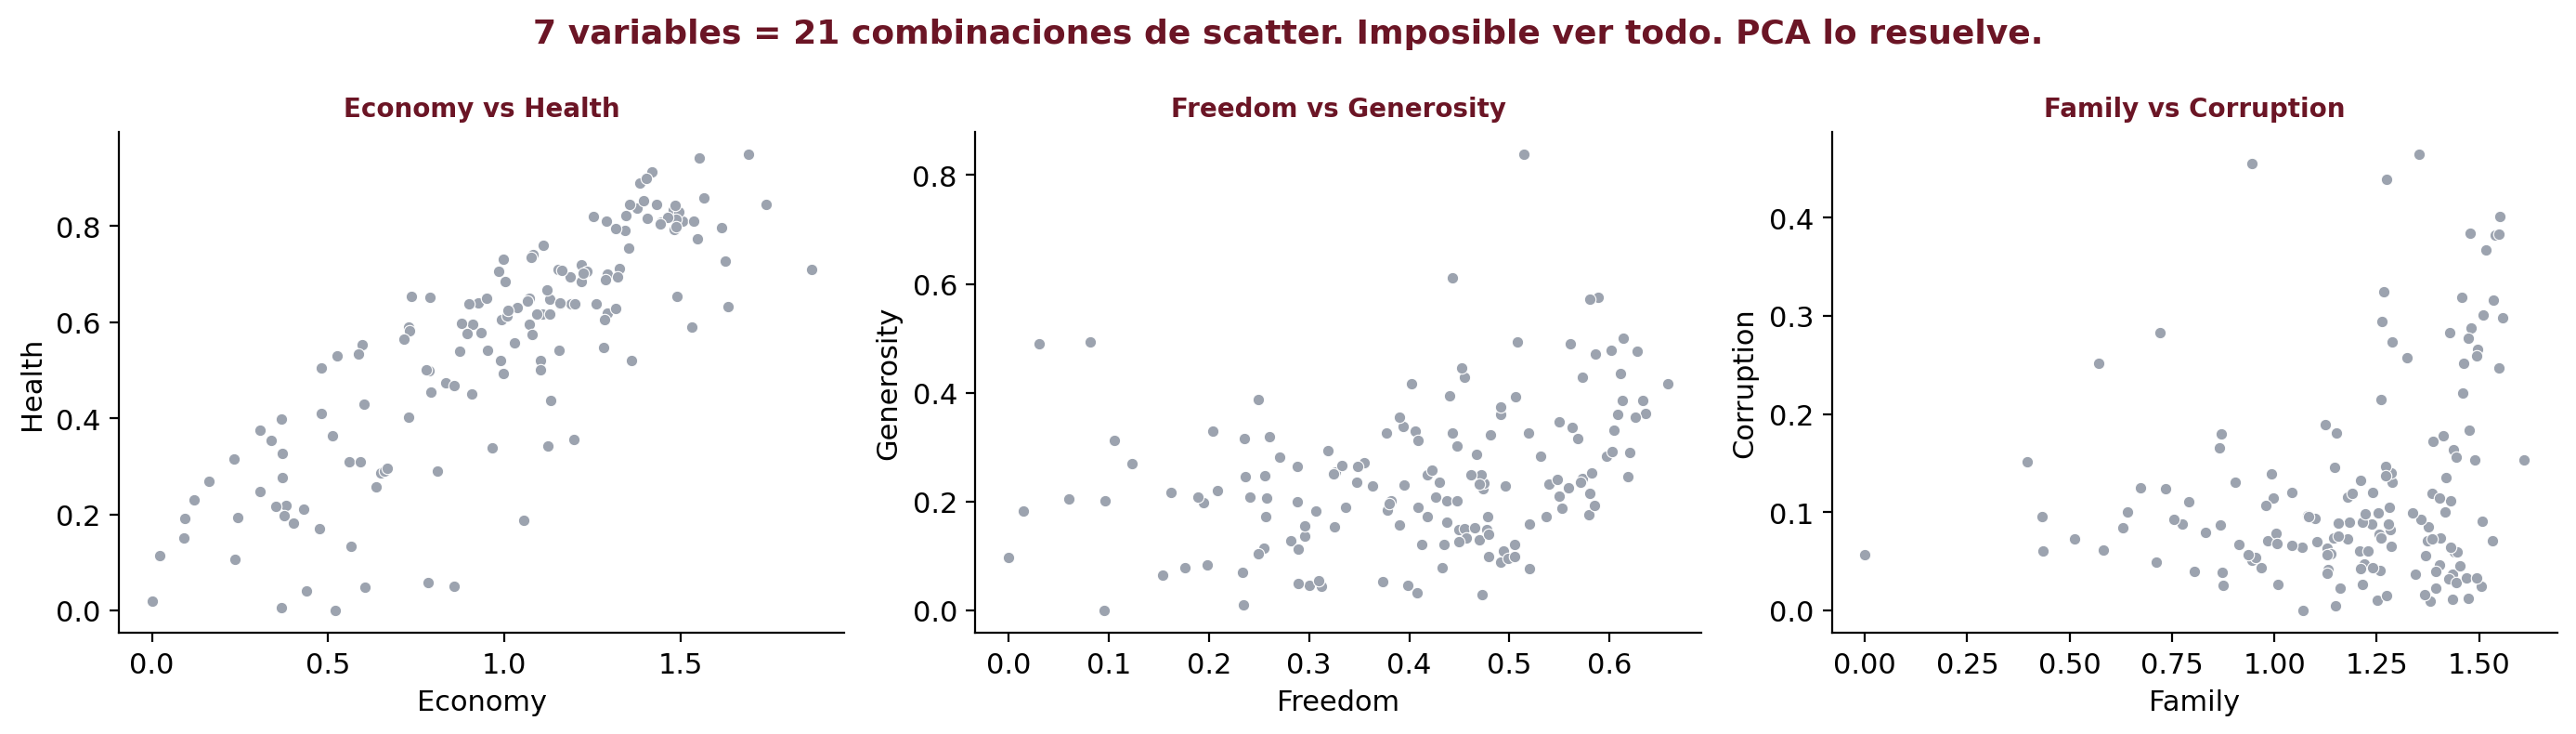
\includegraphics[width=0.95\textwidth]{fig_dimension_problem.png}
  \end{center}

  \vspace{-2pt}
  {\scriptsize\color{textMuted}
    \faLightbulb\hspace{4pt} Tres de los 21 scatters posibles.
    Cada uno muestra solo 2 de 7 variables. Algunos muestran
    patrones, otros no. Necesitamos una forma de ver \textbf{todo}
    en un solo gr\'afico.}
\end{frame}

% =============================================================================
%  BLOQUE B: PCA — LA INTUICI\'ON
% =============================================================================
\sectionframe{PCA}{Comprimir sin perder (mucho)}

\begin{frame}{PCA: La Idea}
  \vspace{-4pt}
  {\footnotesize\color{arcaDark}\bfseries
    PCA (Principal Component Analysis) busca los \textbf{ejes de
    mayor variaci\'on} en los datos y los usa como nuevos ejes.}

  \vspace{6pt}
  {\footnotesize
  \begin{itemize}\setlength{\itemsep}{5pt}
    \item[{\color{arcaRed}\scriptsize\faArrowRight}]
      \textbf{PC1} (primer componente): la direcci\'on en la que los datos
      var\'ian \textbf{m\'as}. Captura la mayor cantidad de informaci\'on.
    \item[{\color{arcaRed}\scriptsize\faArrowRight}]
      \textbf{PC2} (segundo componente): la direcci\'on de m\'axima variaci\'on
      \textbf{perpendicular} a PC1. Captura lo que PC1 no captur\'o.
    \item[{\color{arcaRed}\scriptsize\faArrowRight}]
      \textbf{PC3, PC4\ldots}: cada uno captura menos. Los \'ultimos
      son casi ruido y se pueden descartar.
  \end{itemize}
  }

  \vspace{6pt}
  \begin{tcolorbox}[colback=codeGreen!8, colframe=codeGreen, boxrule=0.5pt, arc=2pt,
    left=6pt, right=6pt, top=4pt, bottom=4pt]
    {\scriptsize\color{arcaDark}
    \faLightbulb\hspace{4pt}\textbf{Resultado:} de 7 variables originales,
    nos quedamos con 2 componentes que capturan el 71\% de la varianza.
    Perdemos 29\%, pero ganamos la capacidad de \textbf{visualizar}
    todos los pa\'ises en un solo scatter.}
  \end{tcolorbox}
\end{frame}

\begin{frame}[shrink=18]{PCA Geom\'etricamente: Rotar los Ejes}
  \vspace{-4pt}
  \begin{center}
    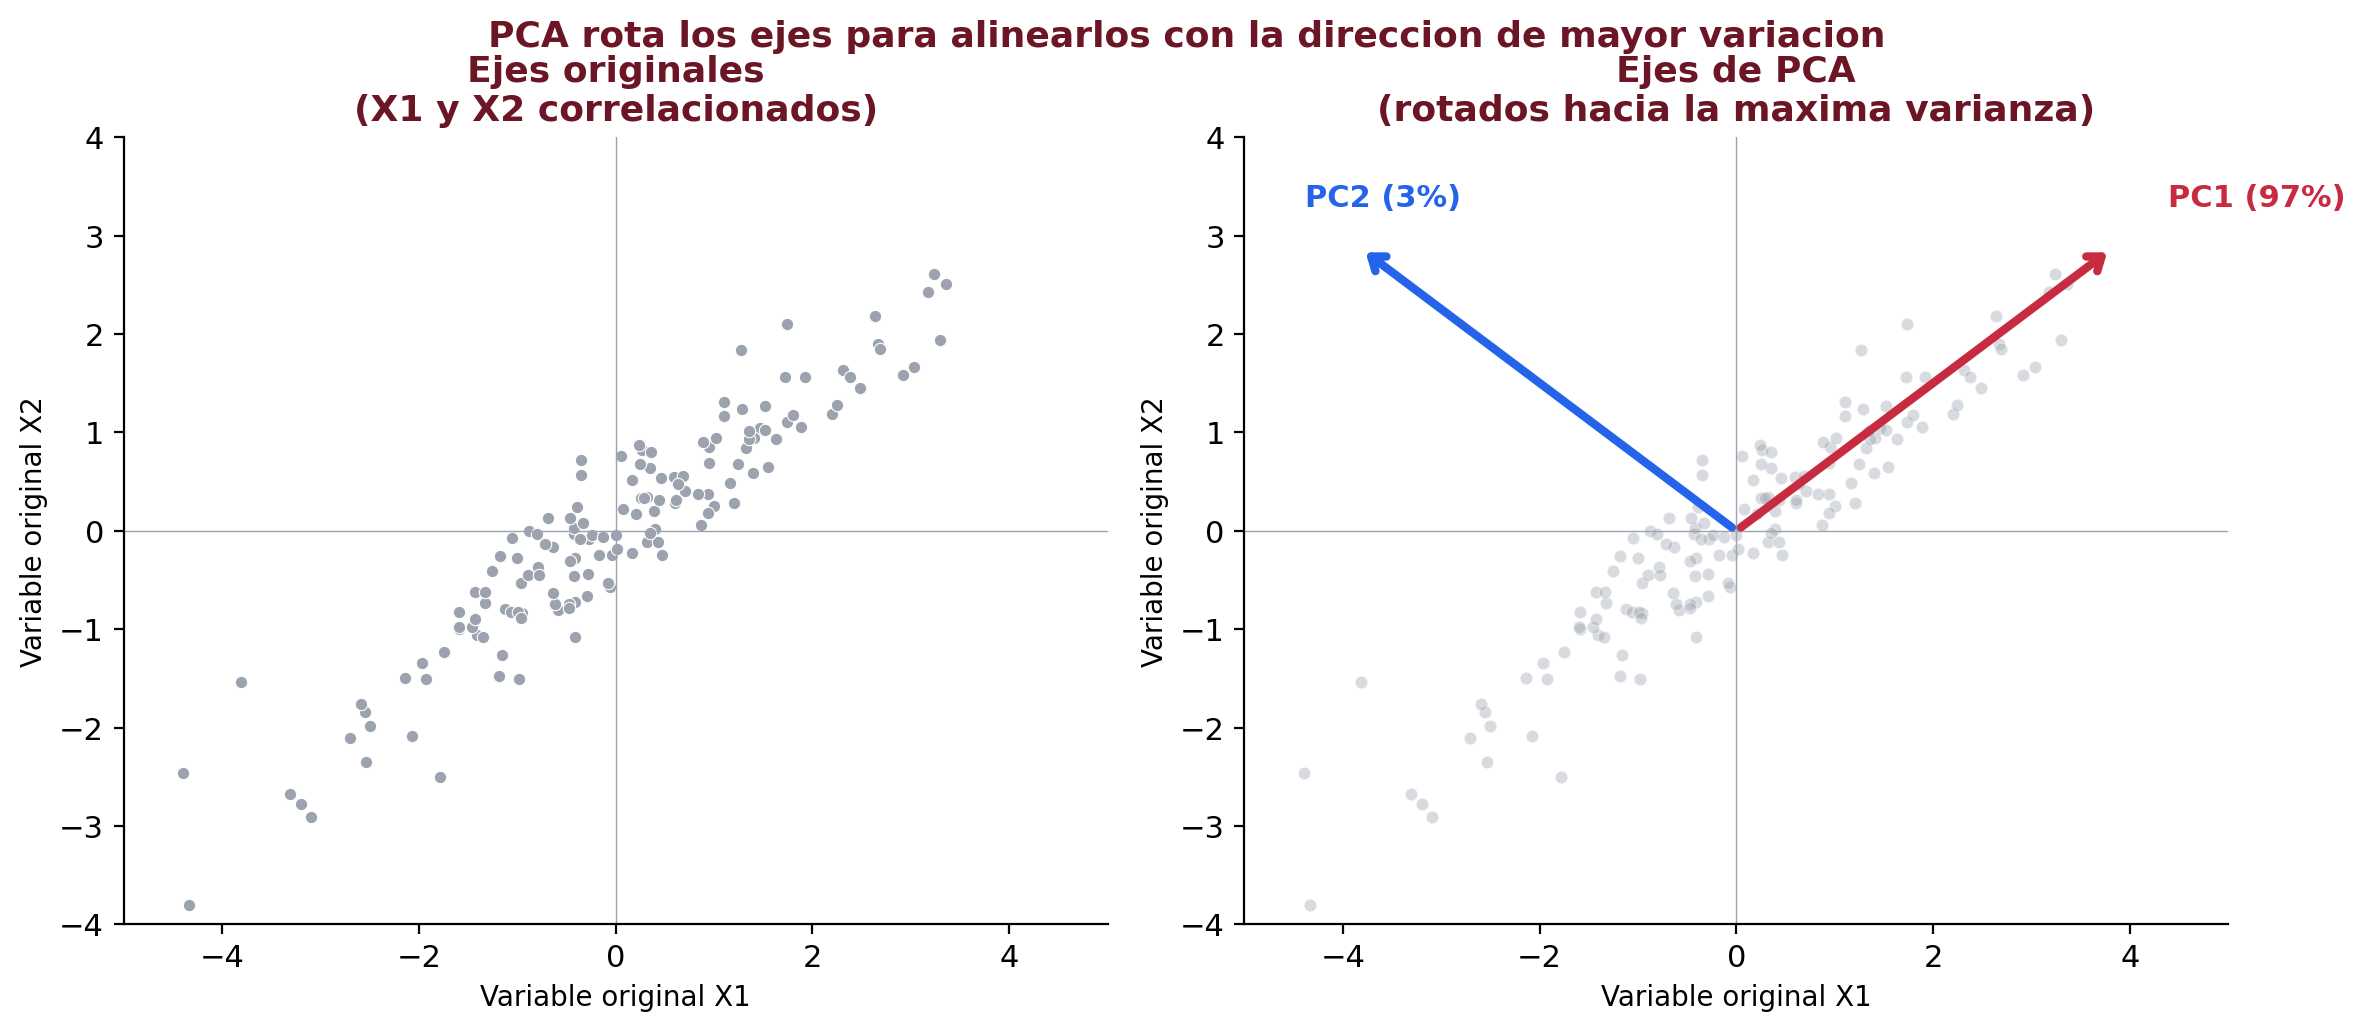
\includegraphics[width=0.88\textwidth]{fig_pca_rotacion.png}
  \end{center}

  \vspace{-2pt}
  {\scriptsize\color{textMuted}
    \faLightbulb\hspace{4pt} \textbf{Izquierda:} datos correlacionados en
    ejes originales (X1, X2). La nube de puntos est\'a inclinada.
    \textbf{Derecha:} PCA rota los ejes para alinearlos con la elipse.
    \textbf{PC1} (rojo) va en la direcci\'on de m\'axima variaci\'on.
    \textbf{PC2} (azul) va perpendicular, capturando lo que queda.}
\end{frame}

\begin{frame}{PCA Paso a Paso --- Conceptual}
  \vspace{-4pt}
  {\footnotesize\color{arcaDark}\bfseries
    Lo que PCA hace internamente (sin entrar en \'algebra lineal):}

  \vspace{6pt}
  {\footnotesize
  \begin{enumerate}\setlength{\itemsep}{5pt}
    \item[{\color{arcaRed}\bfseries 1.}]
      \textbf{Centrar} los datos (restar la media de cada variable).
      El centro de la nube queda en el origen.
    \item[{\color{arcaRed}\bfseries 2.}]
      \textbf{Encontrar} la direcci\'on en la que los datos var\'ian m\'as.
      Esa es PC1. Es una combinaci\'on de las variables originales.
    \item[{\color{arcaRed}\bfseries 3.}]
      \textbf{Encontrar} la direcci\'on perpendicular a PC1 con la
      siguiente mayor varianza. Esa es PC2.
    \item[{\color{arcaRed}\bfseries 4.}]
      Repetir hasta tener tantos componentes como variables originales.
    \item[{\color{codeGreen}\bfseries 5.}]
      \textbf{Descartar} los \'ultimos componentes (los de menor varianza).
      Esos capturan ruido, no patrones reales.
  \end{enumerate}
  }

  \vspace{4pt}
  {\scriptsize\color{textMuted}
    \faLightbulb\hspace{4pt} PCA no inventa informaci\'on.
    \textbf{Reorganiza} la que ya existe para que los primeros
    componentes capturen lo m\'as importante.}
\end{frame}

\begin{frame}{?`Qu\'e Significa ``Varianza Explicada''?}
  \vspace{-4pt}
  {\footnotesize\color{arcaDark}\bfseries
    La varianza total de los datos es fija (100\%).
    PCA la redistribuye entre los componentes:}

  \vspace{6pt}
  {\footnotesize
  \begin{itemize}\setlength{\itemsep}{5pt}
    \item[{\color{arcaRed}\scriptsize\faArrowRight}]
      En los ejes originales, la varianza est\'a \textbf{repartida}
      entre las 7 variables ($\approx$14\% cada una si fueran iguales).
    \item[{\color{codeGreen}\scriptsize\faArrowRight}]
      Despu\'es de PCA, la varianza est\'a \textbf{concentrada}:
      PC1 captura 51.7\%, PC2 el 19.2\%, etc.
    \item[{\color{codeGreen}\scriptsize\faArrowRight}]
      ``PC1 explica el 51.7\% de la varianza'' = si solo usas PC1,
      conservas el 51.7\% de la informaci\'on de las 7 variables originales.
    \item[{\color{arcaRed}\scriptsize\faArrowRight}]
      Lo que descartas (PC5, PC6, PC7) captura solo el 11\% ---
      probablemente ruido.
  \end{itemize}
  }

  \vspace{4pt}
  {\scriptsize\color{textMuted}
    \faLightbulb\hspace{4pt} Varianza = informaci\'on. PCA la concentra
    en los primeros componentes para que puedas descartar los \'ultimos
    sin perder mucho.}
\end{frame}

\begin{frame}[shrink=18]{Elegir 2 Variables a Mano vs PCA}
  \vspace{-4pt}
  \begin{center}
    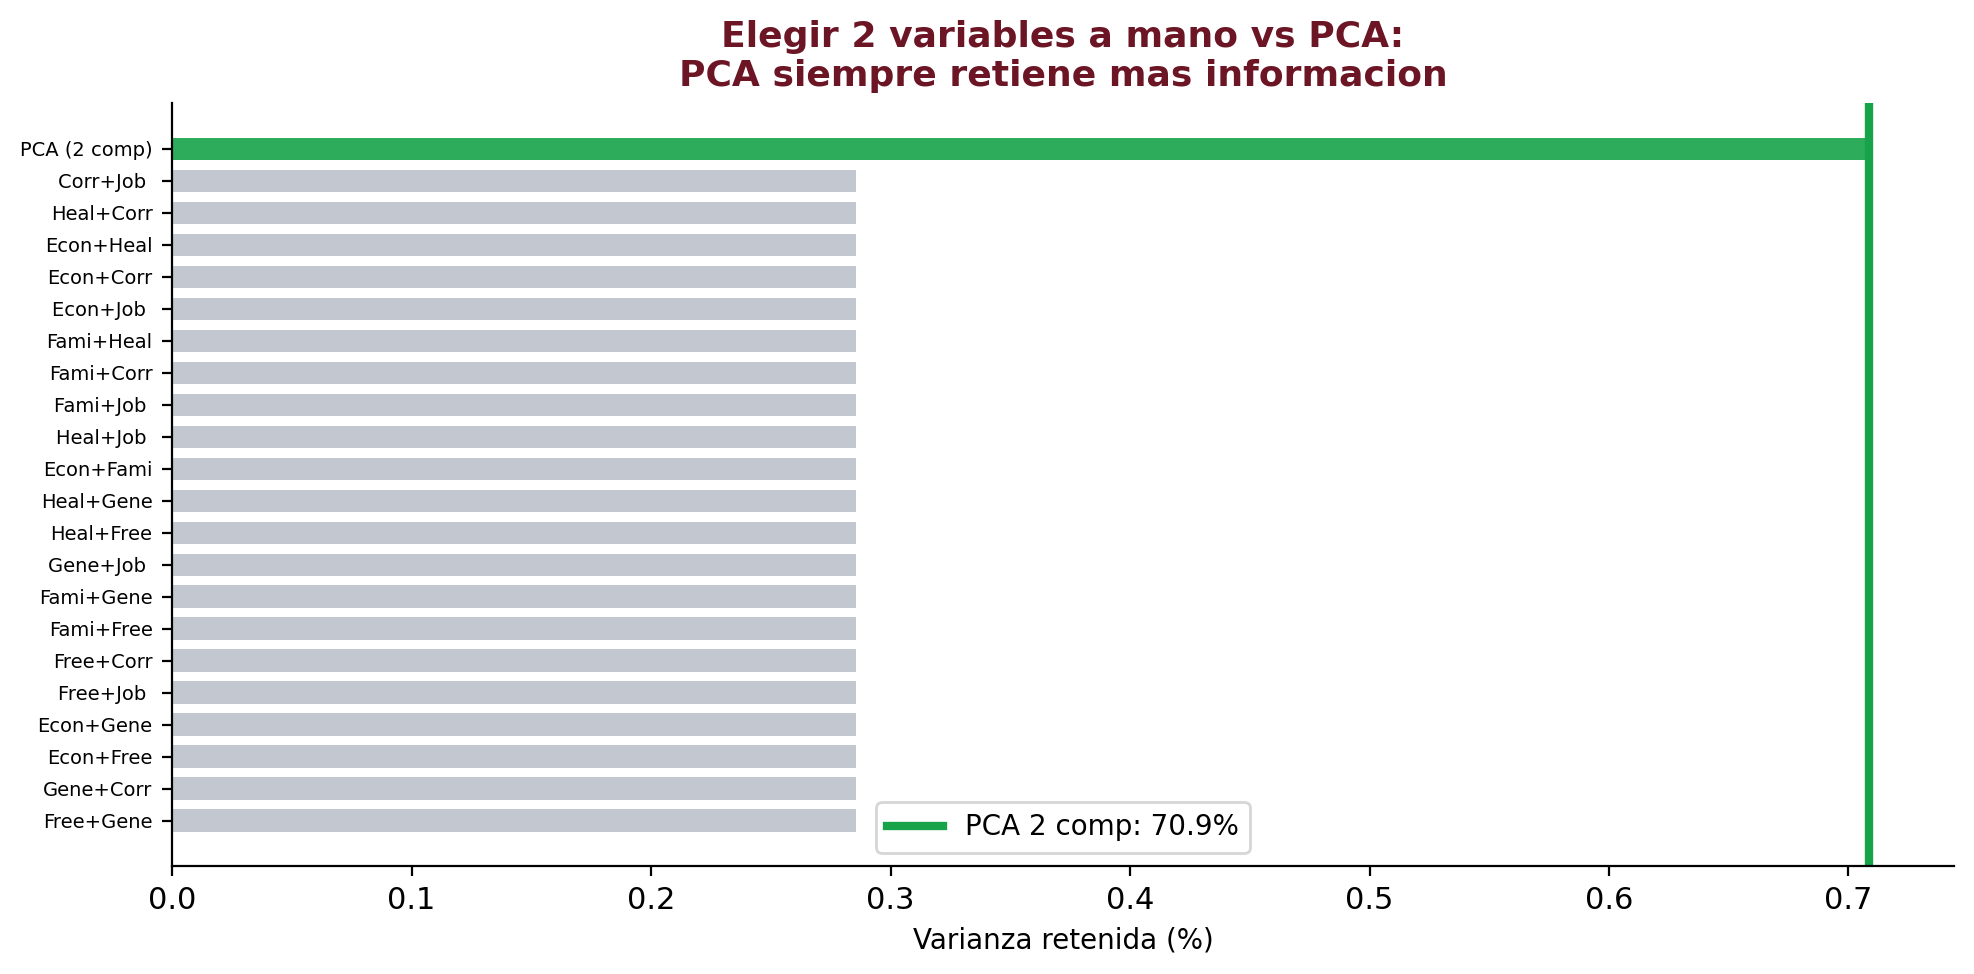
\includegraphics[width=0.78\textwidth]{fig_pca_vs_manual.png}
  \end{center}

  \vspace{-2pt}
  {\scriptsize\color{textMuted}
    \faLightbulb\hspace{4pt} Cada barra gris es una combinaci\'on de 2
    variables originales (21 posibles). La barra verde es PCA con 2
    componentes. \textbf{PCA siempre retiene m\'as informaci\'on} que
    cualquier par de variables originales. Es matem\'aticamente \'optimo.}
\end{frame}

\begin{frame}{PCA para Visualizar vs PCA como Preprocesamiento}
  \vspace{-4pt}
  {\footnotesize\color{arcaDark}\bfseries
    PCA se usa con dos prop\'ositos distintos:}

  \vspace{6pt}
  {\scriptsize
  \begin{tabular}{@{}p{3.5cm}p{4.5cm}p{4.5cm}@{}}
    \toprule
     & \textbf{\color{codeBlue}Para visualizar} & \textbf{\color{arcaRed}Como preprocesamiento} \\
    \midrule
    \textbf{Componentes} & 2 o 3 (para scatter). & Los que den $\geq$ 80\% de varianza. \\
    \textbf{Objetivo} & Ver patrones, clusters, outliers en un scatter. & Quitar ruido antes de un modelo (K-Means, RF, etc.). \\
    \textbf{Ejemplo} & El biplot de hoy: 7 vars $\to$ 2D. & 100 features $\to$ 20 componentes antes de RF. \\
    \textbf{Trade-off} & Perdemos varianza (29\%), pero vemos todo. & Perdemos poco (20\%), pero el modelo es m\'as r\'apido y robusto. \\
    \bottomrule
  \end{tabular}
  }

  \vspace{6pt}
  {\scriptsize\color{textMuted}
    \faLightbulb\hspace{4pt} Hoy usamos PCA para \textbf{ambas cosas}:
    visualizar los 151 pa\'ises en 2D, y luego aplicar K-Means sobre
    los 2 componentes (preprocesamiento que elimina ruido).}
\end{frame}

\begin{frame}{?`Qu\'e Asume PCA?}
  \vspace{-4pt}
  {\footnotesize\color{arcaDark}\bfseries
    PCA funciona bien bajo ciertas condiciones:}

  \vspace{6pt}
  {\scriptsize
  \begin{tabular}{@{}p{3.5cm}p{4cm}p{4.5cm}@{}}
    \toprule
    \textbf{Supuesto} & \textbf{Qu\'e espera} & \textbf{Consecuencia} \\
    \midrule
    \textbf{Variables num\'ericas} & Todas continuas. & No funciona con categ\'oricas directamente. \\
    \textbf{Escalas comparables} & Misma escala o escaladas. & \textbf{StandardScaler obligatorio} (igual que K-Means). \\
    \textbf{Relaciones lineales} & Las variables est\'an correlacionadas linealmente. & Si la relaci\'on es no lineal, PCA no la captura bien. \\
    \textbf{Varianza = informaci\'on} & M\'as varianza = m\'as informaci\'on. & Descarta componentes de baja varianza (``ruido''). \\
    \bottomrule
  \end{tabular}
  }

  \vspace{6pt}
  {\scriptsize\color{textMuted}
    \faLightbulb\hspace{4pt} PCA es una \textbf{transformaci\'on lineal}.
    Rota los ejes para alinearlos con la direcci\'on de mayor varianza.
    No inventa informaci\'on --- la reorganiza.}
\end{frame}

\begin{frame}[fragile,shrink=18]{C\'odigo: PCA en sklearn}
  \vspace{-6pt}
  \begin{pyblock}
from sklearn.decomposition import PCA
from sklearn.preprocessing import StandardScaler

features = ["Economy", "Family", "Health", "Freedom",
            "Generosity", "Corruption", "Job Satisfaction"]
X = df[features].dropna()

scaler = StandardScaler()
X_scaled = scaler.fit_transform(X)

pca = PCA(n_components=2)
X_pca = pca.fit_transform(X_scaled)

print(f"Original: {X.shape}")        # (151, 7)
print(f"PCA:      {X_pca.shape}")     # (151, 2)
print(f"Varianza: {pca.explained_variance_ratio_.sum():.1%}")
  \end{pyblock}

  \vspace{4pt}
  {\scriptsize\color{arcaDark}
    \faKey\hspace{4pt} De 7 columnas a 2. El 71\% de la varianza
    original se conserva. Ahora podemos hacer un scatter de 151
    pa\'ises en 2D.}
\end{frame}

% =============================================================================
%  BLOQUE C: SCREE PLOT
% =============================================================================
\sectionframe{Scree Plot}{?`Cu\'antos componentes conservar?}

\begin{frame}[shrink=18]{Varianza Explicada por Componente}
  \vspace{-4pt}
  \begin{center}
    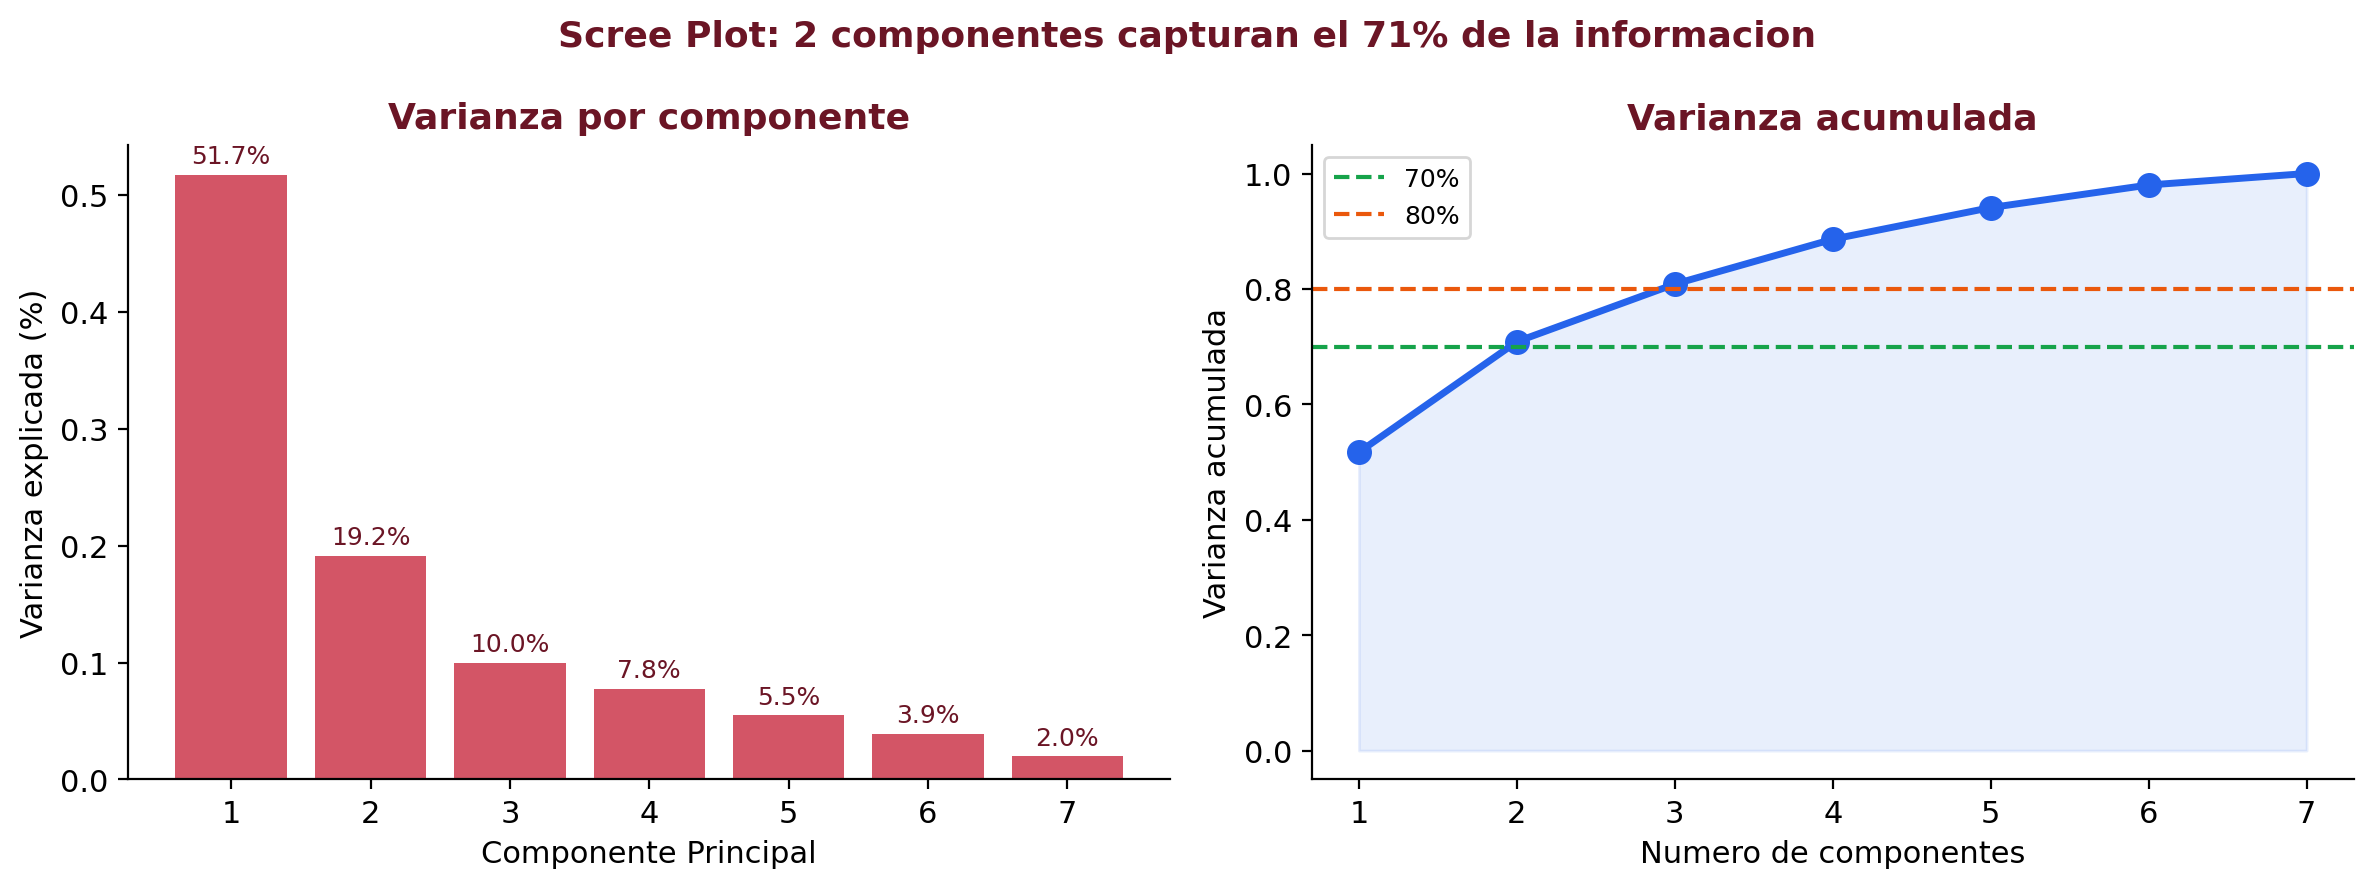
\includegraphics[width=0.88\textwidth]{fig_scree.png}
  \end{center}

  \vspace{-2pt}
  {\scriptsize\color{textMuted}
    \faLightbulb\hspace{4pt} \textbf{Izquierda:} PC1 sola captura el
    51.7\%. PC2 agrega 19.2\%. Los dem\'as aportan poco cada uno.
    \textbf{Derecha:} con 2 componentes llegamos a 71\%, con 3 a 81\%.
    El ``codo'' est\'a en 2--3 componentes.}
\end{frame}

\begin{frame}{?`Cu\'antos Elegir? --- Criterios}
  \vspace{-4pt}
  {\footnotesize\color{arcaDark}\bfseries
    No hay una regla \'unica. Tres criterios comunes:}

  \vspace{6pt}
  {\footnotesize
  \begin{enumerate}\setlength{\itemsep}{5pt}
    \item[{\color{arcaRed}\bfseries 1.}]
      \textbf{Varianza acumulada $\geq$ 70--80\%:} conservar suficientes
      componentes para explicar al menos el 70\% de la varianza.
      Con 2 componentes tenemos 71\% --- suficiente.
    \item[{\color{arcaRed}\bfseries 2.}]
      \textbf{Codo en el scree plot:} similar al m\'etodo del codo de
      K-Means. Donde la curva deja de bajar r\'apido.
    \item[{\color{arcaRed}\bfseries 3.}]
      \textbf{Objetivo pr\'actico:} si queremos \textbf{visualizar},
      necesitamos 2 o 3 componentes (para scatter 2D o 3D).
      Si queremos reducir ruido antes de un modelo, m\'as.
  \end{enumerate}
  }

  \vspace{4pt}
  {\scriptsize\color{textMuted}
    \faLightbulb\hspace{4pt} Para esta clase, usamos \textbf{2 componentes}:
    suficiente varianza (71\%) y permite un scatter 2D interpretable.}
\end{frame}

% =============================================================================
%  BLOQUE D: INTERPRETAR COMPONENTES
% =============================================================================
\sectionframe{Interpretar los Componentes}{?`Qu\'e significa PC1 y PC2?}

\begin{frame}{Loadings: El ADN de Cada Componente}
  \vspace{-4pt}
  {\footnotesize\color{arcaDark}\bfseries
    Cada componente principal es una \textbf{combinaci\'on lineal} de las
    variables originales. Los \textbf{loadings} dicen cu\'anto pesa cada
    variable en cada componente.}

  \vspace{6pt}
  {\footnotesize
  \begin{itemize}\setlength{\itemsep}{4pt}
    \item[{\color{arcaRed}\scriptsize\faArrowRight}]
      Si Economy tiene loading alto en PC1, significa que PC1
      captura mucha de la variaci\'on en Economy.
    \item[{\color{arcaRed}\scriptsize\faArrowRight}]
      Si Generosity tiene loading alto en PC2 pero bajo en PC1,
      significa que la generosidad var\'ia en una direcci\'on
      \textbf{independiente} del desarrollo econ\'omico.
    \item[{\color{codeGreen}\scriptsize\faArrowRight}]
      Los loadings permiten \textbf{nombrar} los componentes:
      PC1 = ``desarrollo'', PC2 = ``libertad y confianza social''.
  \end{itemize}
  }

  \vspace{4pt}
  {\scriptsize\color{textMuted}
    \faLightbulb\hspace{4pt} Los loadings son los coeficientes de la
    transformaci\'on. Se acceden con \texttt{pca.components\_}.}
\end{frame}

\begin{frame}[shrink=15]{Heatmap de Loadings}
  \vspace{-4pt}
  \begin{center}
    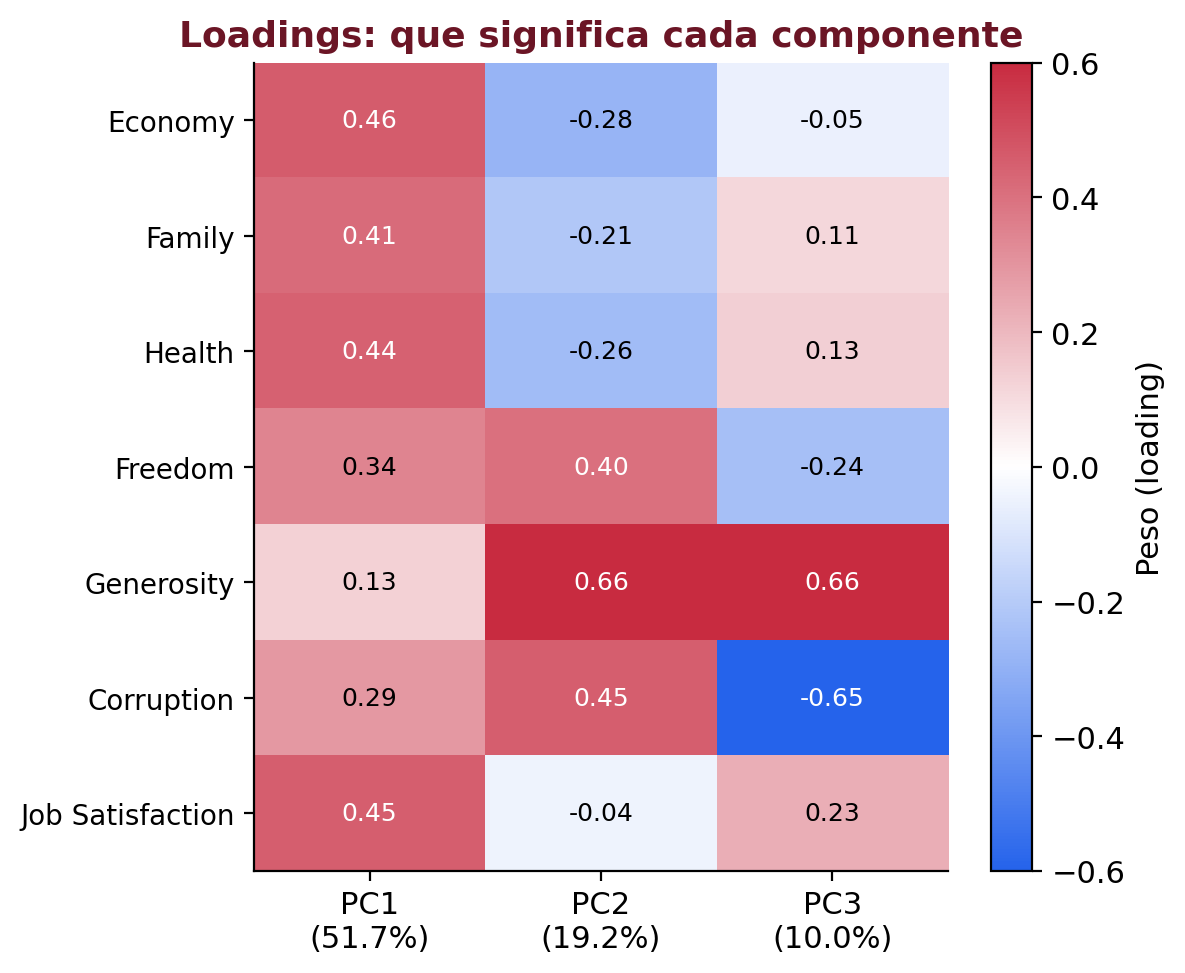
\includegraphics[width=0.5\textwidth]{fig_loadings.png}
  \end{center}

  \vspace{-2pt}
  {\scriptsize\color{textMuted}
    \faLightbulb\hspace{4pt} \textbf{PC1:} Economy, Health, Job Satisfaction
    y Family pesan fuerte $\to$ es un eje de \textbf{desarrollo y calidad
    de vida}. \textbf{PC2:} Generosity, Corruption y Freedom dominan
    $\to$ es un eje de \textbf{libertad y confianza social}.
    Noruega est\'a arriba-derecha (alto en ambos). Chad est\'a abajo-izquierda.}
\end{frame}

\begin{frame}[shrink=22]{Biplot: Pa\'ises + Flechas de Loadings}
  \vspace{-4pt}
  \begin{center}
    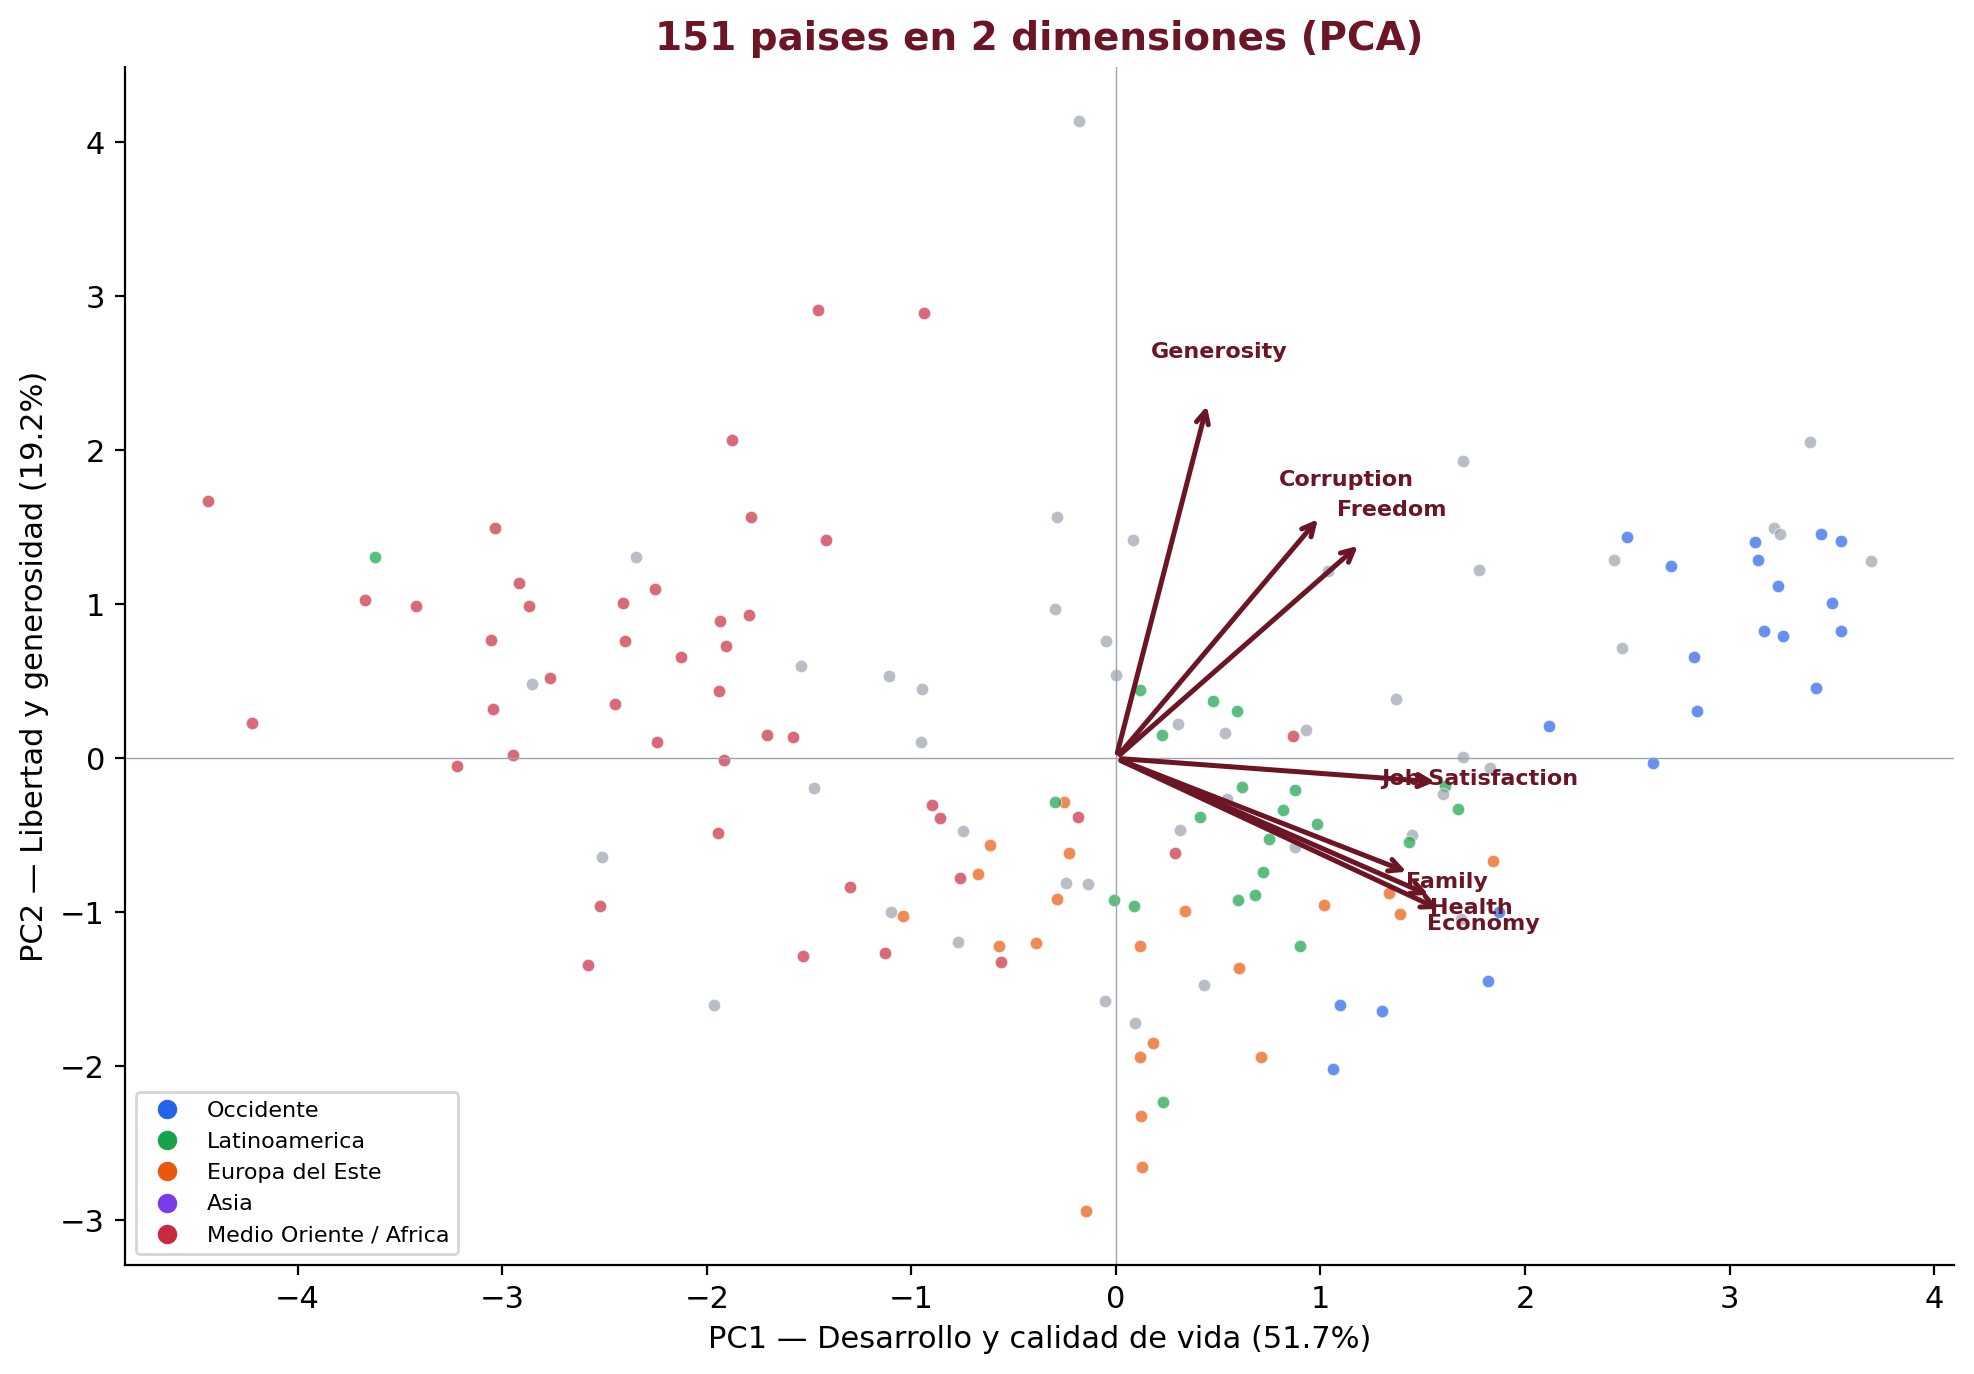
\includegraphics[width=0.78\textwidth]{fig_biplot.png}
  \end{center}

  \vspace{-2pt}
  {\scriptsize\color{textMuted}
    \faLightbulb\hspace{4pt} Cada punto es un pa\'is. Las flechas muestran
    hacia d\'onde ``apuntan'' las variables. Economy, Health y Family
    apuntan a la derecha (PC1). Generosity y Freedom apuntan arriba (PC2).
    Los pa\'ises de Occidente est\'an a la derecha. \'Africa a la izquierda.}
\end{frame}

\begin{frame}[fragile,shrink=18]{Explorar el Espacio PCA con Plotly}
  \vspace{-6pt}
  \begin{pyblock}
df["PC1"] = X_pca[:, 0]
df["PC2"] = X_pca[:, 1]

fig = px.scatter(df, x="PC1", y="PC2", color="Region",
    hover_data=["Country", "Happiness Score"],
    title="151 paises en 2D (PCA)",
    labels={"PC1": "PC1 - Desarrollo (51.7%)",
            "PC2": "PC2 - Libertad (19.2%)"},
    opacity=0.8)
fig.update_layout(template="plotly_white")
fig.show()
  \end{pyblock}

  \vspace{4pt}
  {\scriptsize\color{arcaDark}
    \faMousePointer\hspace{4pt} Pasen el mouse sobre cada punto:
    ven el pa\'is y su Happiness Score.
    Noruega est\'a arriba-derecha (alto desarrollo + alta libertad).
    Chad abajo-izquierda (bajo en ambos).
    Ecuador en la zona media, con otros latinoamericanos.}
\end{frame}

\begin{frame}[fragile,shrink=10]{Scatter 3D con 3 Componentes}
  \vspace{-4pt}
  {\footnotesize\color{arcaDark}\bfseries
    Con 3 componentes capturamos el 81\% de la varianza:}

  \vspace{4pt}
  \begin{pyblock}
pca3 = PCA(n_components=3)
X_pca3 = pca3.fit_transform(X_scaled)
df["PC3"] = X_pca3[:, 2]

fig = px.scatter_3d(df, x="PC1", y="PC2", z="PC3",
    color="Region", hover_data=["Country", "Happiness Score"],
    title="151 paises en 3D (81% de varianza)",
    opacity=0.7)
fig.update_layout(template="plotly_white")
fig.show()
  \end{pyblock}

  \vspace{4pt}
  {\scriptsize\color{textMuted}
    \faMousePointer\hspace{4pt} Roten con el mouse.
    PC3 agrega un 10\% --- separa pa\'ises que en 2D se solapaban.}
\end{frame}

% =============================================================================
%  BLOQUE E: PCA + K-MEANS
% =============================================================================
\sectionframe{PCA + K-Means}{El pipeline completo}

\begin{frame}{?`Por Qu\'e Combinarlos?}
  \vspace{-4pt}
  {\footnotesize\color{arcaDark}\bfseries
    Usar K-Means directamente sobre 7 variables funciona, pero
    tiene problemas. PCA antes mejora todo:}

  \vspace{6pt}
  {\footnotesize
  \begin{itemize}\setlength{\itemsep}{5pt}
    \item[{\color{arcaRed}\scriptsize\faTimesCircle}]
      \textbf{Sin PCA:} K-Means en 7D. No podemos visualizar los
      clusters. Variables ruidosas confunden al algoritmo.
    \item[{\color{codeGreen}\scriptsize\faCheckCircle}]
      \textbf{Con PCA:} reducir a 2--3 dimensiones elimina ruido.
      K-Means en 2D produce clusters m\'as limpios y
      \textbf{visualizables}.
    \item[{\color{codeGreen}\scriptsize\faCheckCircle}]
      PCA act\'ua como un \textbf{filtro de ruido}: las \'ultimas
      componentes (las que descartamos) suelen capturar ruido,
      no patrones reales.
  \end{itemize}
  }

  \vspace{6pt}
  \begin{tcolorbox}[colback=arcaGray, colframe=arcaRed, boxrule=0.5pt, arc=2pt,
    left=6pt, right=6pt, top=4pt, bottom=4pt]
    {\scriptsize\color{arcaDark}
    \faKey\hspace{4pt}\textbf{Pipeline:}
    datos originales $\to$ \texttt{StandardScaler}
    $\to$ \texttt{PCA(n\_components=2)}
    $\to$ \texttt{KMeans(n\_clusters=3)}
    $\to$ interpretar.}
  \end{tcolorbox}
\end{frame}

\begin{frame}[fragile,shrink=22]{C\'odigo: El Pipeline Completo}
  \vspace{-6pt}
  \begin{pyblock}
from sklearn.pipeline import Pipeline

pipeline = Pipeline([
    ("scaler", StandardScaler()),
    ("pca", PCA(n_components=2)),
    ("kmeans", KMeans(n_clusters=3, random_state=42, n_init=10)),
])

df["cluster"] = pipeline.fit_predict(X)

# Ver que paises hay en cada cluster
for c in range(3):
    paises = df[df["cluster"] == c]["Country"].tolist()
    score = df[df["cluster"] == c]["Happiness Score"].mean()
    print(f"Cluster {c} ({len(paises)} paises, "
          f"felicidad={score:.1f}): {paises[:5]}...")
  \end{pyblock}

  \vspace{4pt}
  {\scriptsize\color{arcaDark}
    \faKey\hspace{4pt} \texttt{Pipeline} encadena los pasos en una sola
    l\'inea. Escala, reduce y segmenta de un solo golpe.}
\end{frame}

\begin{frame}[shrink=22]{PCA + K-Means --- Visual}
  \vspace{-4pt}
  \begin{center}
    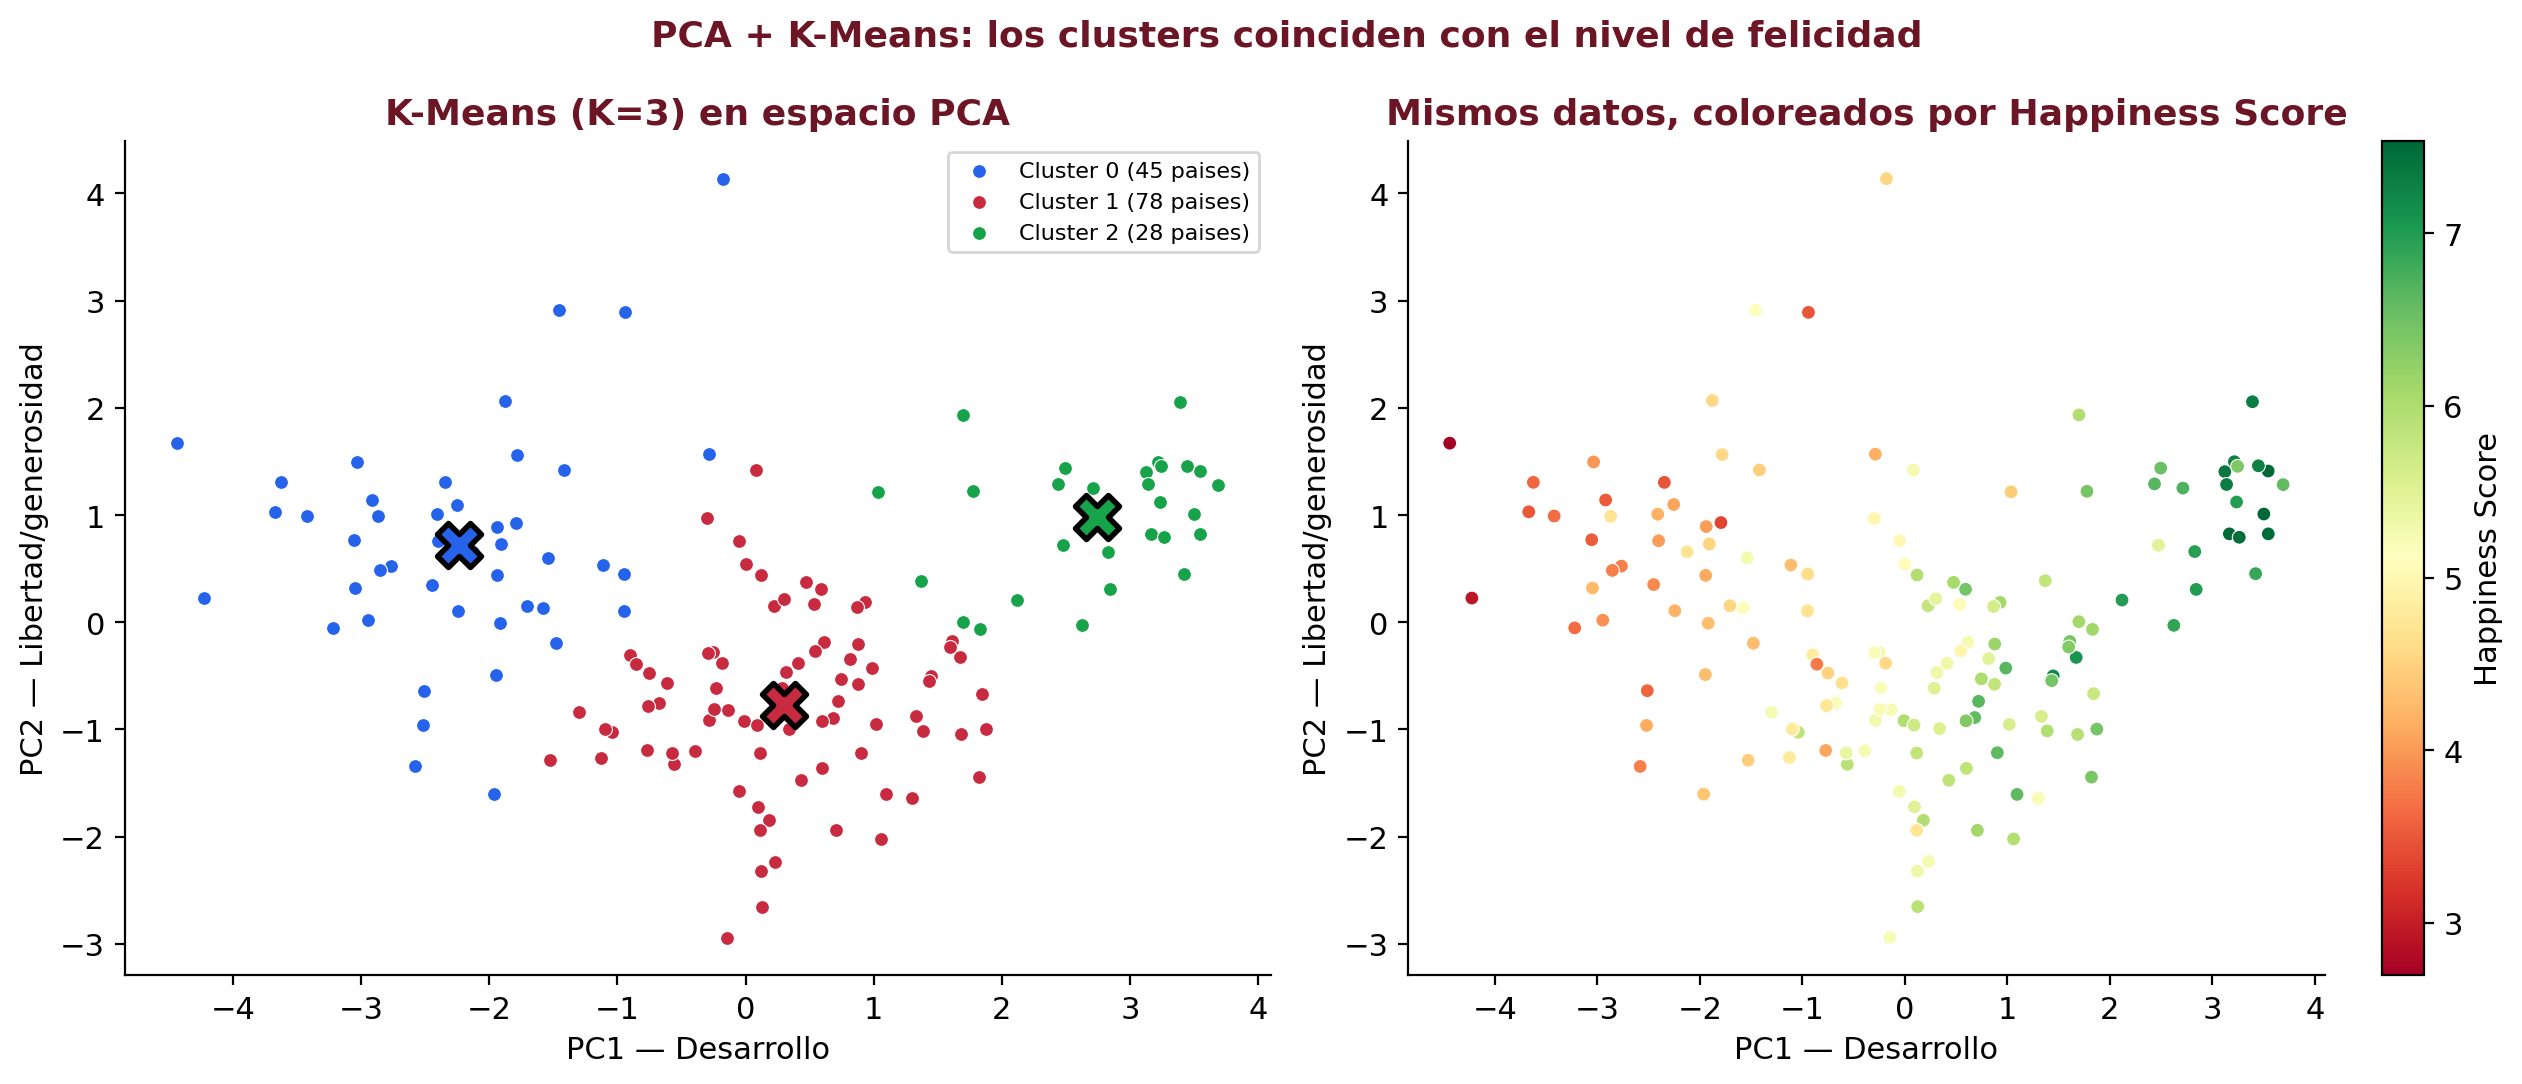
\includegraphics[width=0.95\textwidth]{fig_pca_kmeans.png}
  \end{center}

  \vspace{-2pt}
  {\scriptsize\color{textMuted}
    \faLightbulb\hspace{4pt} \textbf{Izquierda:} 3 clusters en el espacio
    PCA. Se ven claramente separados.
    \textbf{Derecha:} los mismos datos coloreados por Happiness Score.
    Los clusters \textbf{coinciden} con el nivel de felicidad: el cluster
    verde (derecha) son los pa\'ises m\'as felices.}
\end{frame}

\begin{frame}[shrink=15]{Antes y Despu\'es de PCA}
  \vspace{-4pt}
  \begin{center}
    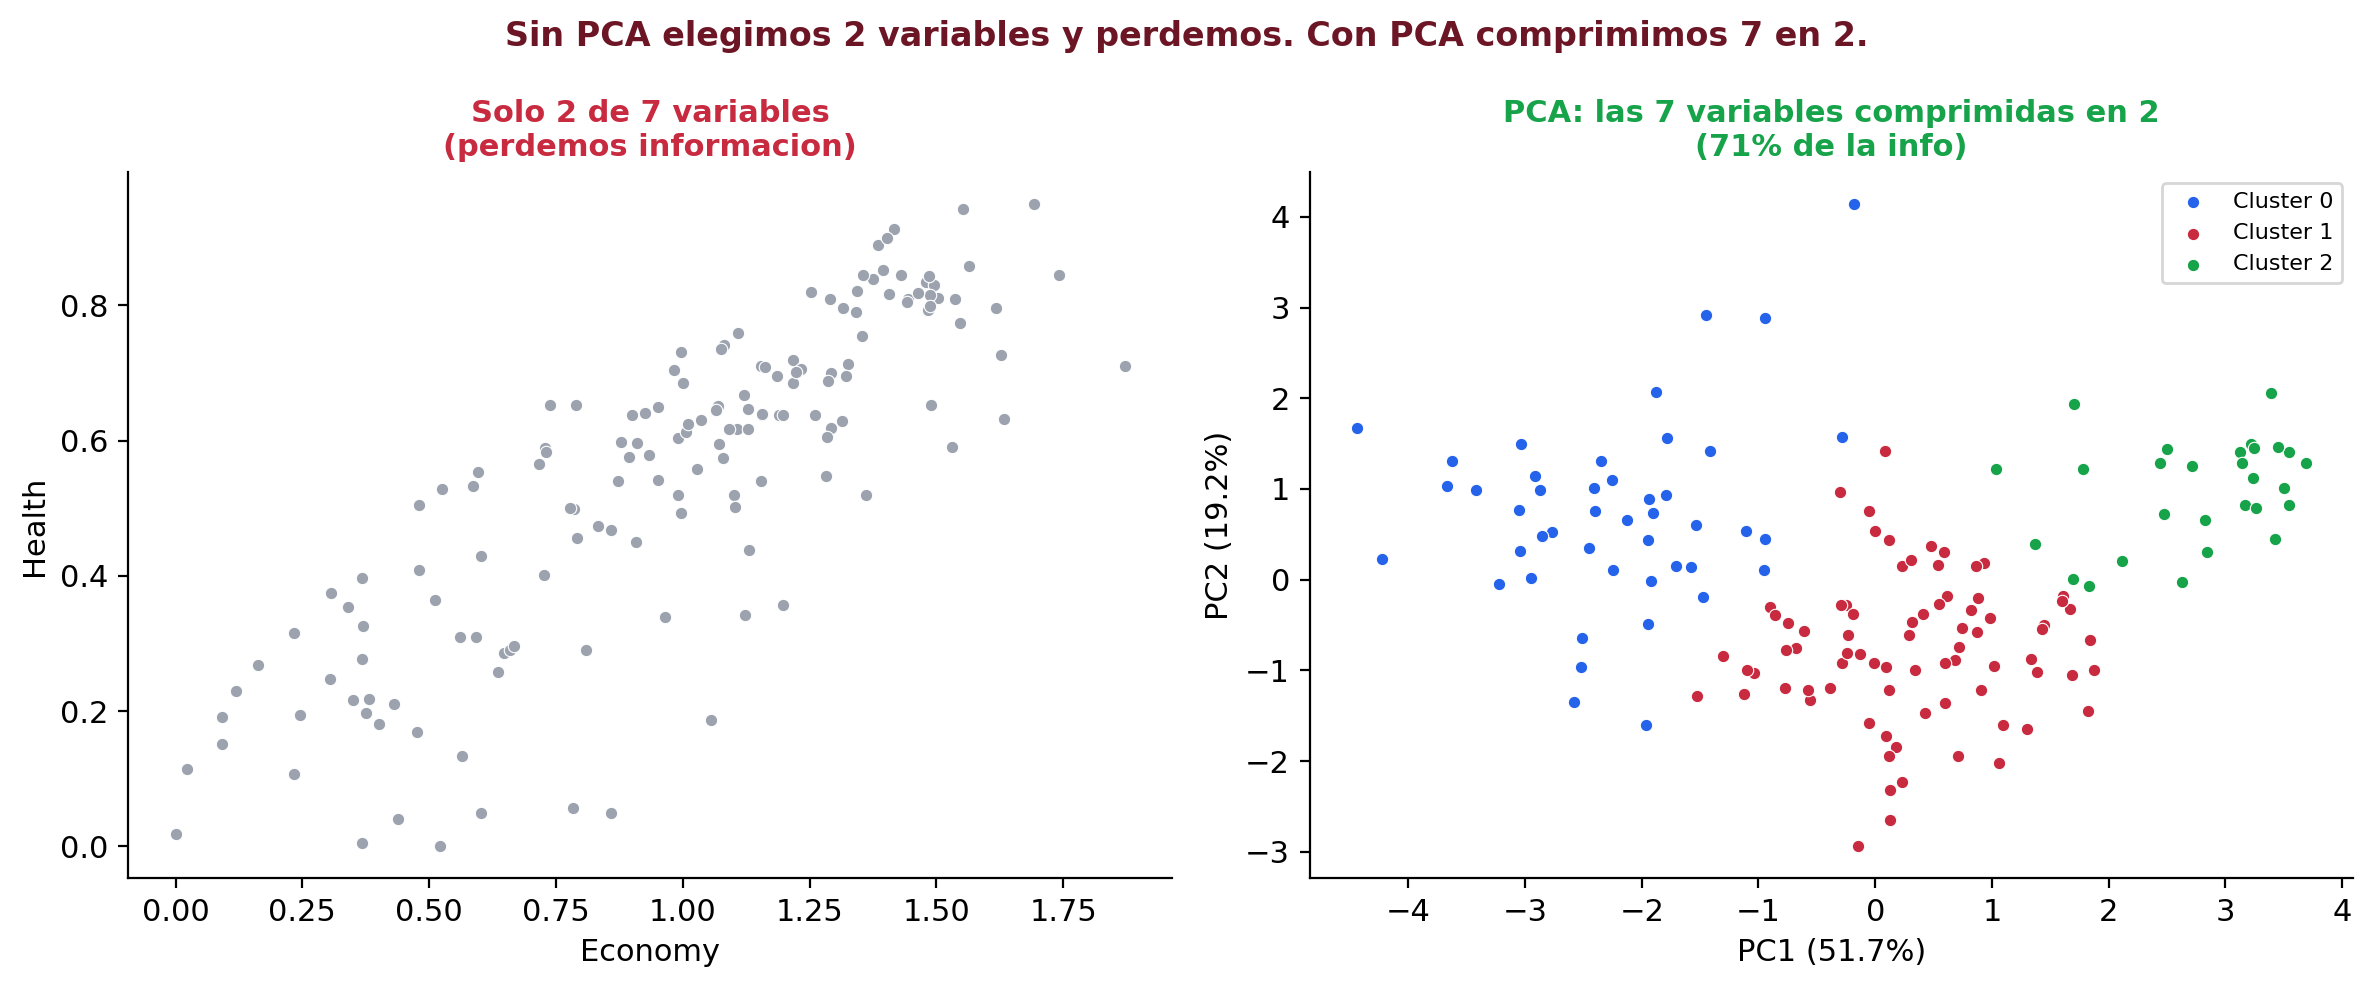
\includegraphics[width=0.88\textwidth]{fig_antes_despues.png}
  \end{center}

  \vspace{-2pt}
  {\scriptsize\color{textMuted}
    \faLightbulb\hspace{4pt} \textbf{Sin PCA:} elegimos 2 de 7 variables
    (Economy vs Health) y perdemos las otras 5.
    \textbf{Con PCA:} las 7 variables est\'an comprimidas en 2 componentes.
    Los clusters son m\'as claros porque usan \textbf{toda} la informaci\'on.}
\end{frame}

% =============================================================================
%  BLOQUE F: INTERPRETACI\'ON
% =============================================================================
\sectionframe{Interpretaci\'on}{?`Qu\'e define la felicidad de un pa\'is?}

\begin{frame}[fragile,shrink=18]{Perfilar los Clusters}
  \vspace{-6pt}
  \begin{pyblock}
perfil = df.groupby("cluster")[
    ["Happiness Score"] + features
].mean().round(2)
print(perfil)
  \end{pyblock}

  \vspace{4pt}
  {\scriptsize\color{arcaDark}
  \begin{itemize}\setlength{\itemsep}{3pt}
    \item[{\color{codeGreen}\scriptsize\faArrowRight}]
      \textbf{Cluster ``Desarrollados'':} Economy, Health y
      Job Satisfaction altos. Felicidad $\approx$ 6.8.
    \item[{\color{codeOrange}\scriptsize\faArrowRight}]
      \textbf{Cluster ``Transici\'on'':} valores medios en todo.
      Felicidad $\approx$ 5.6.
    \item[{\color{arcaRed}\scriptsize\faArrowRight}]
      \textbf{Cluster ``En desarrollo'':} indicadores bajos.
      Felicidad $\approx$ 4.1.
  \end{itemize}
  }
\end{frame}

\begin{frame}{?`Qu\'e Aprendimos sobre la Felicidad?}
  \vspace{-4pt}
  {\footnotesize\color{arcaDark}\bfseries
    PCA revel\'o que la felicidad de un pa\'is se explica principalmente
    por dos ejes:}

  \vspace{6pt}
  {\footnotesize
  \begin{itemize}\setlength{\itemsep}{5pt}
    \item[{\color{codeBlue}\bfseries PC1}]
      \textbf{Desarrollo material} (51.7\%): econom\'ia, salud, familia,
      satisfacci\'on laboral. Es el factor dominante. Los pa\'ises con
      mayor desarrollo material son m\'as felices en promedio.
    \item[{\color{codePurple}\bfseries PC2}]
      \textbf{Libertad y confianza} (19.2\%): libertad, generosidad,
      (baja) corrupci\'on. Explica por qu\'e pa\'ises con econom\'ia
      similar tienen felicidad distinta.
  \end{itemize}
  }

  \vspace{6pt}
  \begin{tcolorbox}[colback=arcaGray, colframe=arcaRed, boxrule=0.5pt, arc=2pt,
    left=6pt, right=6pt, top=4pt, bottom=4pt]
    {\scriptsize\color{arcaDark}
    \faKey\hspace{4pt}\textbf{Interpretaci\'on:} el dinero importa (PC1),
    pero no lo es todo. La libertad y la confianza social (PC2)
    explican casi el 20\% de la variaci\'on en felicidad ---
    pa\'ises ricos pero corruptos son menos felices de lo esperado.}
  \end{tcolorbox}
\end{frame}

\begin{frame}[shrink=5]{Ejercicio: Aplicar PCA + K-Means a Mall Customers}
  \vspace{-4pt}
  {\footnotesize\color{arcaDark}\bfseries
    \faClock\hspace{4pt} 15 minutos --- en el notebook:}

  \vspace{6pt}
  {\footnotesize
  \begin{enumerate}\setlength{\itemsep}{4pt}
    \item Cargar Mall Customers (clase 19). Usar Age, income, spending.
    \item Escalar + PCA con 2 componentes. ?`Cu\'anta varianza se conserva?
    \item Scatter PCA coloreado por cluster de K-Means.
    \item Comparar: con 3 variables originales, ?`PCA aporta mucho?
    \item ?`Qu\'e variable domina PC1? ?`Y PC2?
    \item \textbf{Reflexi\'on:} ?`cu\'ando vale la pena PCA y cu\'ando no?
  \end{enumerate}
  }
\end{frame}

% =============================================================================
%  BLOQUE G: t-SNE --- CUANDO PCA NO ALCANZA
% =============================================================================
\sectionframe{t-SNE}{Cuando PCA no alcanza}

\begin{frame}{PCA Es Lineal --- A Veces No Basta}
  \vspace{-4pt}
  {\footnotesize\color{arcaDark}\bfseries
    PCA busca ejes rectos (combinaciones lineales). Pero si la estructura
    de los datos es \textbf{curva o compleja}, una proyecci\'on lineal
    no la captura bien.}

  \vspace{6pt}
  {\footnotesize
  \begin{itemize}\setlength{\itemsep}{5pt}
    \item[{\color{arcaRed}\scriptsize\faArrowRight}]
      Con 7 variables de Happiness, PCA funciona bien (71\% en 2D).
      La estructura es aproximadamente lineal.
    \item[{\color{arcaRed}\scriptsize\faArrowRight}]
      Con 64 pixeles de una imagen de un d\'igito, la relaci\'on entre
      pixeles es \textbf{altamente no lineal}. PCA en 2D pierde mucho
      y los d\'igitos se solapan.
    \item[{\color{codeGreen}\scriptsize\faArrowRight}]
      \textbf{t-SNE} (t-distributed Stochastic Neighbor Embedding):
      un algoritmo \textbf{no lineal} que preserva las
      \textbf{relaciones de vecindad} --- puntos cercanos en alta
      dimensi\'on quedan cercanos en 2D.
  \end{itemize}
  }
\end{frame}

\begin{frame}{t-SNE: ?`Qu\'e Hace Diferente?}
  \vspace{-4pt}
  {\scriptsize
  \begin{tabular}{@{}p{3.5cm}p{4.5cm}p{4.5cm}@{}}
    \toprule
     & \textbf{\color{codeBlue}PCA} & \textbf{\color{codePurple}t-SNE} \\
    \midrule
    \textbf{Tipo} & Lineal. & No lineal. \\
    \textbf{Preserva} & Estructura \textbf{global} (distancias grandes). & \textbf{Vecindarios} (puntos cercanos). \\
    \textbf{Param\'etrico} & S\'i: tiene \texttt{.transform()} para datos nuevos. & \textbf{No}: solo transforma los datos de entrada. No puede proyectar datos nuevos. \\
    \textbf{Varianza explicada} & S\'i: sabemos cu\'anto captura cada PC. & \textbf{No}: no tiene m\'etrica de ``varianza''. \\
    \textbf{Reproducible} & S\'i: siempre da el mismo resultado. & Depende de \texttt{random\_state} y \texttt{perplexity}. \\
    \textbf{Velocidad} & R\'apido (incluso con 100K filas). & Lento (minutos con $>$ 10K filas). \\
    \textbf{Mejor para} & Preprocesamiento, reducci\'on de ruido. & \textbf{Visualizaci\'on} de alta dimensi\'on. \\
    \bottomrule
  \end{tabular}
  }

  \vspace{6pt}
  \begin{tcolorbox}[colback=arcaRed!8, colframe=arcaRed, boxrule=0.5pt, arc=2pt,
    left=6pt, right=6pt, top=4pt, bottom=4pt]
    {\scriptsize\color{arcaDark}
    \faExclamationTriangle\hspace{4pt}\textbf{Cuidado con t-SNE:}
    los ejes no tienen significado (no hay ``loadings'').
    Las distancias entre clusters lejanos no son confiables.
    Solo las relaciones \textbf{locales} (vecinos) son v\'alidas.
    Usarlo para \textbf{explorar}, no para medir.}
  \end{tcolorbox}
\end{frame}

\begin{frame}{?`C\'omo Ve una Computadora una Imagen?}
  \vspace{-4pt}
  {\footnotesize\color{arcaDark}\bfseries
    Una imagen \textbf{no es una foto} para la m\'aquina. Es una
    \textbf{matriz de n\'umeros}, donde cada n\'umero es la intensidad
    de un \textbf{pixel}.}

  \vspace{6pt}
  {\scriptsize
  \begin{tabular}{@{}lll p{4.6cm}@{}}
    \toprule
    \textbf{Tipo} & \textbf{Forma} & \textbf{Rango} & \textbf{Ejemplo} \\
    \midrule
    Grises  & $H \times W$           & 0 (negro) -- 255 (blanco) & Foto 100$\times$100 = 10\,000 n\'umeros \\
    RGB     & $H \times W \times 3$  & 0--255 por canal           & Foto 100$\times$100 = 30\,000 n\'umeros \\
    RGBA    & $H \times W \times 4$  & + canal de transparencia   & PNG con fondo transparente \\
    \bottomrule
  \end{tabular}
  }

  \vspace{6pt}
  \begin{center}
    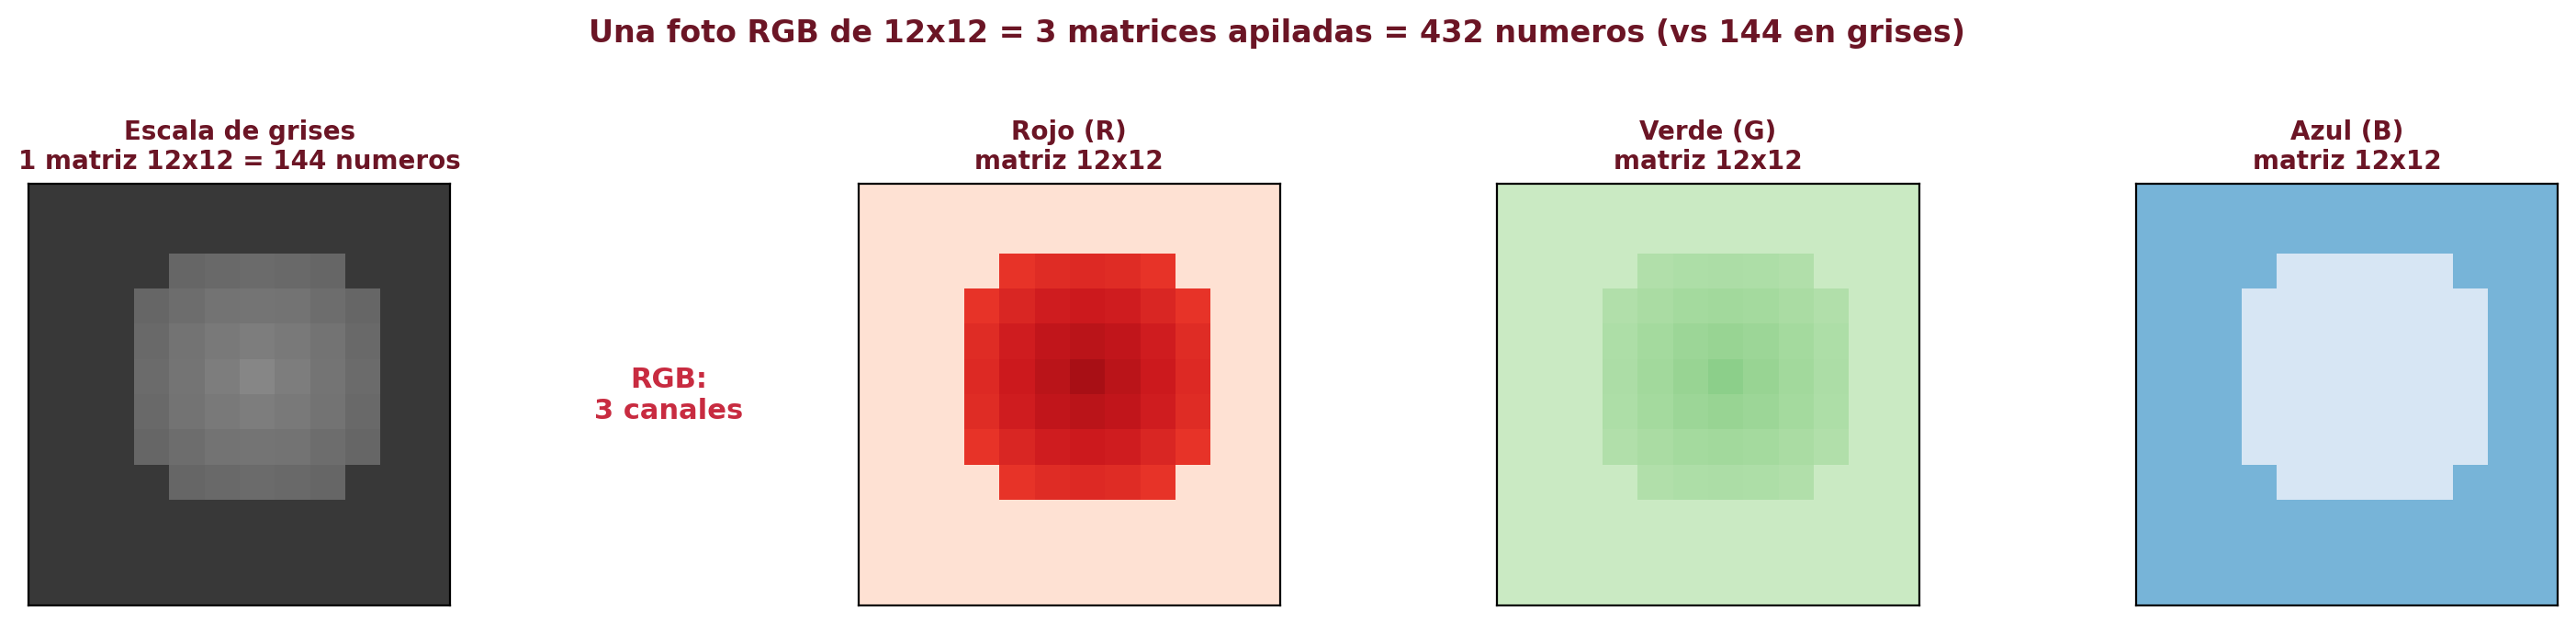
\includegraphics[width=0.95\textwidth]{fig_imagen_rgb.png}
  \end{center}

  \vspace{-2pt}
  {\scriptsize\color{textMuted}
    \faLightbulb\hspace{4pt} Una imagen RGB es \textbf{tres matrices apiladas}.
    El color de cada pixel = mezcla de R, G y B. La m\'aquina solo ve n\'umeros.}
\end{frame}

\begin{frame}[shrink=10]{De Imagen a Vector: \texttt{.flatten()}}
  \vspace{-4pt}
  {\footnotesize\color{arcaDark}\bfseries
    Para usar una imagen en ML la \textbf{aplanamos}: la matriz 2D se
    convierte en un \textbf{vector 1D} --- una fila del DataFrame con
    tantas columnas como pixeles.}

  \vspace{4pt}
  \begin{center}
    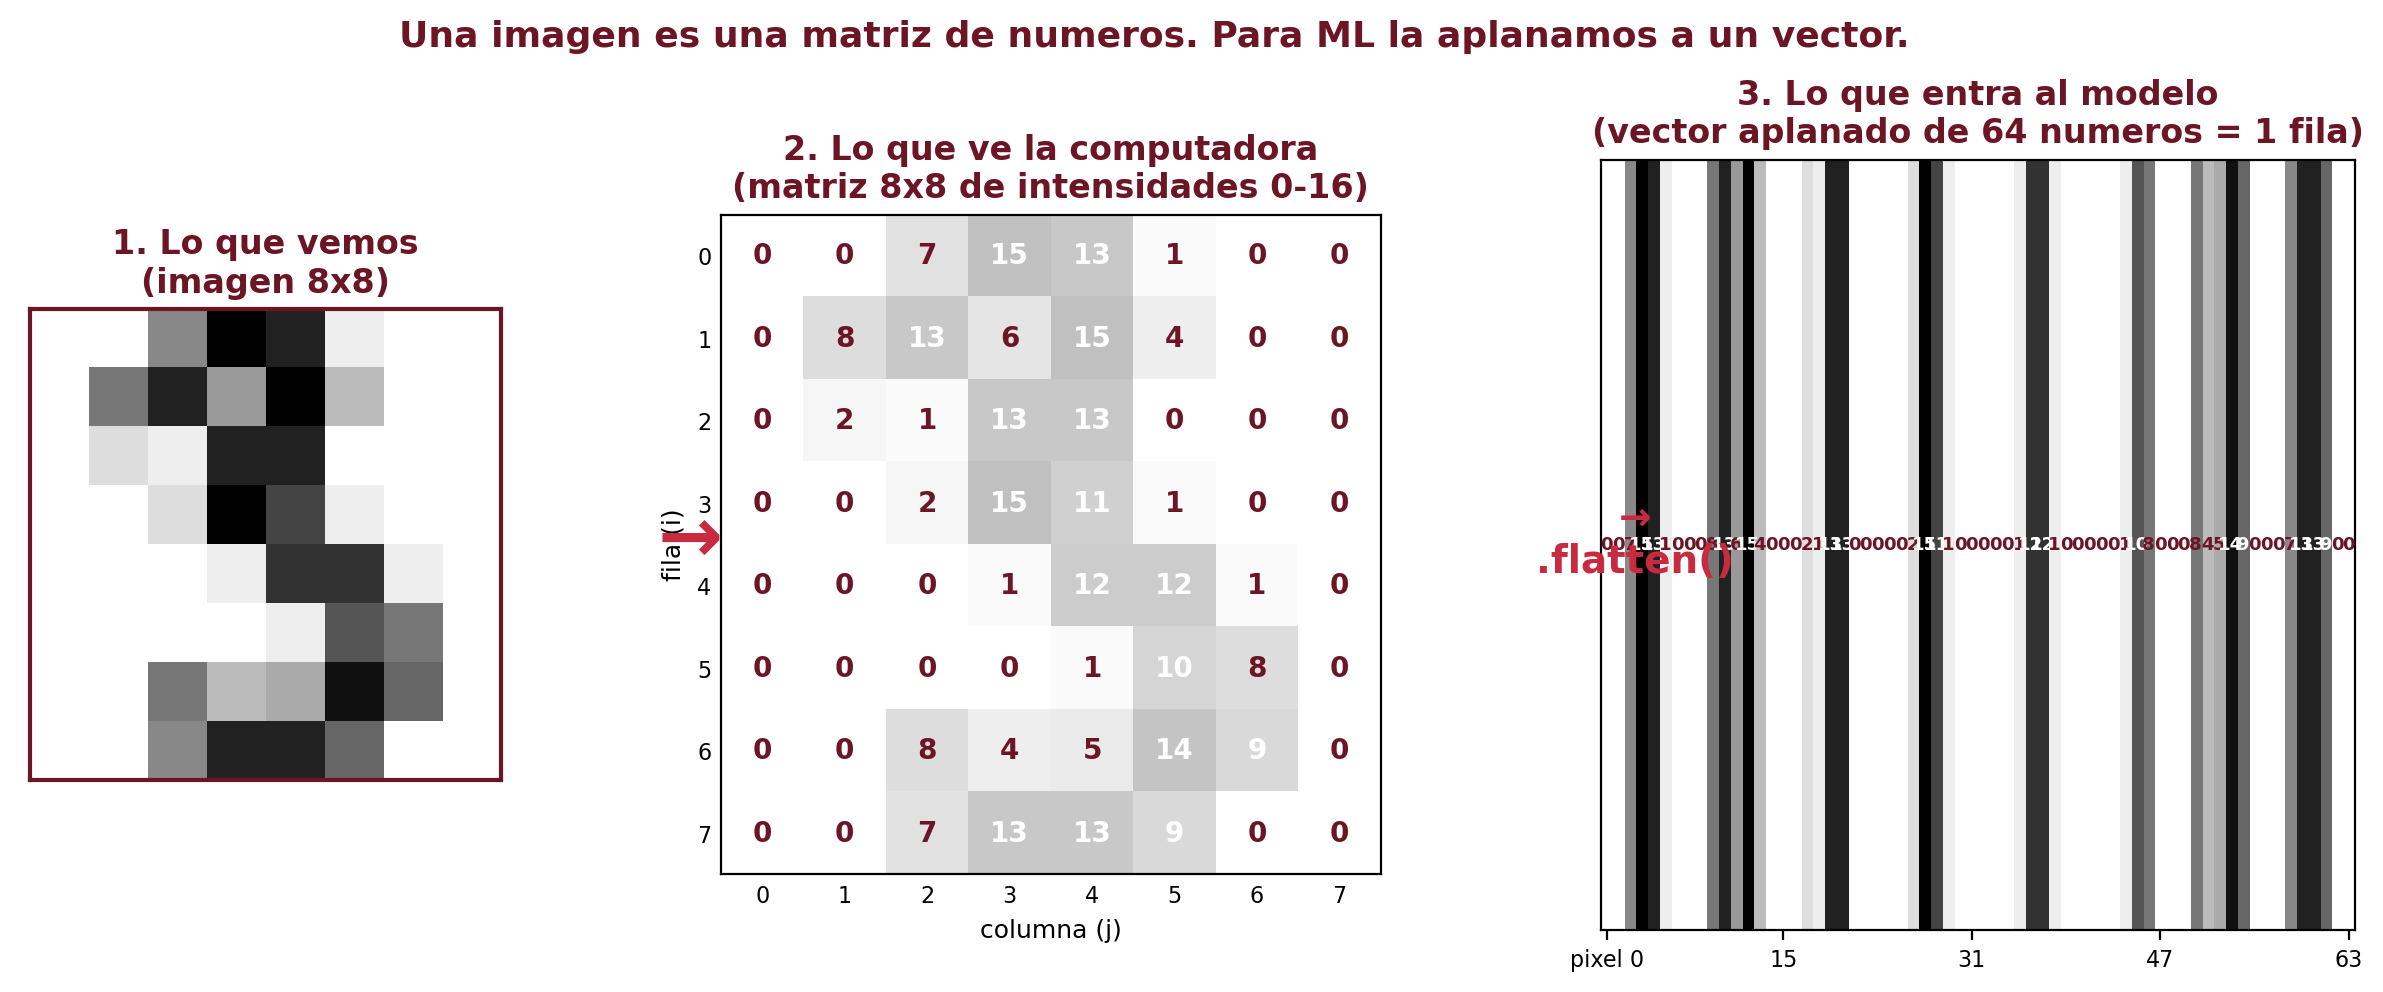
\includegraphics[width=0.97\textwidth]{fig_imagen_a_vector.png}
  \end{center}

  \vspace{-2pt}
  {\scriptsize\color{textMuted}
    \faLightbulb\hspace{4pt} 1797 d\'igitos $\times$ 64 pixeles =
    DataFrame de \textbf{1797 filas $\times$ 64 columnas}. Las columnas
    no son ``edad'' ni ``ingreso'' --- son posiciones de pixel.
    Cualquier modelo (PCA, K-Means, Random Forest) trabaja exactamente
    igual que con datos tabulares.}
\end{frame}

\begin{frame}[fragile,shrink=12]{Cargar una Imagen Real en Python}
  \vspace{-4pt}
  {\footnotesize\color{arcaDark}\bfseries
    \texttt{matplotlib.pyplot.imread()} lee cualquier imagen
    (PNG, JPG) y devuelve un array de NumPy listo para usar.}

  \vspace{4pt}
  \begin{pyblock}
import matplotlib.pyplot as plt
import numpy as np

img = plt.imread("foto.jpg")     # array NumPy
print(img.shape)                  # (alto, ancho, 3) si es RGB
print(img.dtype, img.min(), img.max())   # uint8 0..255

plt.imshow(img); plt.axis("off"); plt.show()  # mostrar

gris = img.mean(axis=2)           # promedio R,G,B -> grises (alto, ancho)
vector = gris.flatten()           # 1 fila para ML: alto*ancho numeros
  \end{pyblock}

  \vspace{4pt}
  {\scriptsize\color{arcaDark}
  \begin{itemize}\setlength{\itemsep}{2pt}
    \item[{\color{arcaRed}\scriptsize\faArrowRight}]
      \textbf{\texttt{plt.imread}} \emph{(matplotlib)}: r\'apido, sin
      instalar nada extra. Devuelve \texttt{float} (PNG) o \texttt{uint8} (JPG).
    \item[{\color{arcaRed}\scriptsize\faArrowRight}]
      \textbf{\texttt{PIL.Image.open}} \emph{(Pillow)}: m\'as opciones
      (resize, convert a grises con \texttt{.convert("L")}, rotar).
    \item[{\color{codeGreen}\scriptsize\faArrowRight}]
      Para meter \textbf{N im\'agenes} en un dataset:
      \texttt{np.stack([plt.imread(f).flatten() for f in files])}.
  \end{itemize}
  }
\end{frame}

\begin{frame}{El Dataset: D\'igitos Escritos a Mano}
  \vspace{-4pt}
  {\footnotesize\color{arcaDark}\bfseries
    \texttt{load\_digits()} de sklearn: 1797 im\'agenes de n\'umeros
    escritos a mano, cada una de $8 \times 8$ pixeles. Versi\'on reducida
    del cl\'asico \textbf{MNIST} (28$\times$28, 70\,000 im\'agenes, desde 1998).}

  \vspace{6pt}
  {\scriptsize
  \begin{tabular}{@{}llp{7cm}@{}}
    \toprule
    \textbf{Propiedad} & \textbf{Valor} & \textbf{Significado} \\
    \midrule
    Observaciones & 1\,797 & Im\'agenes de d\'igitos 0--9. \\
    Variables & 64 & Cada pixel es una variable (intensidad 0--16). \\
    Clases & 10 & Los d\'igitos 0, 1, 2, \ldots, 9. \\
    \bottomrule
  \end{tabular}
  }

  \vspace{6pt}
  {\footnotesize
  \begin{itemize}\setlength{\itemsep}{4pt}
    \item[{\color{arcaRed}\scriptsize\faArrowRight}]
      Cada fila del dataset es una imagen \textbf{aplanada}:
      8$\times$8 = 64 n\'umeros. No son variables ``normales''
      como edad o ingreso --- son \textbf{pixeles}.
    \item[{\color{arcaRed}\scriptsize\faArrowRight}]
      El objetivo: ver si podemos distinguir los 10 d\'igitos
      en un scatter 2D, sin usar las etiquetas.
  \end{itemize}
  }
\end{frame}

\begin{frame}[shrink=18]{As\'i Se Ven los D\'igitos}
  \vspace{-4pt}
  \begin{center}
    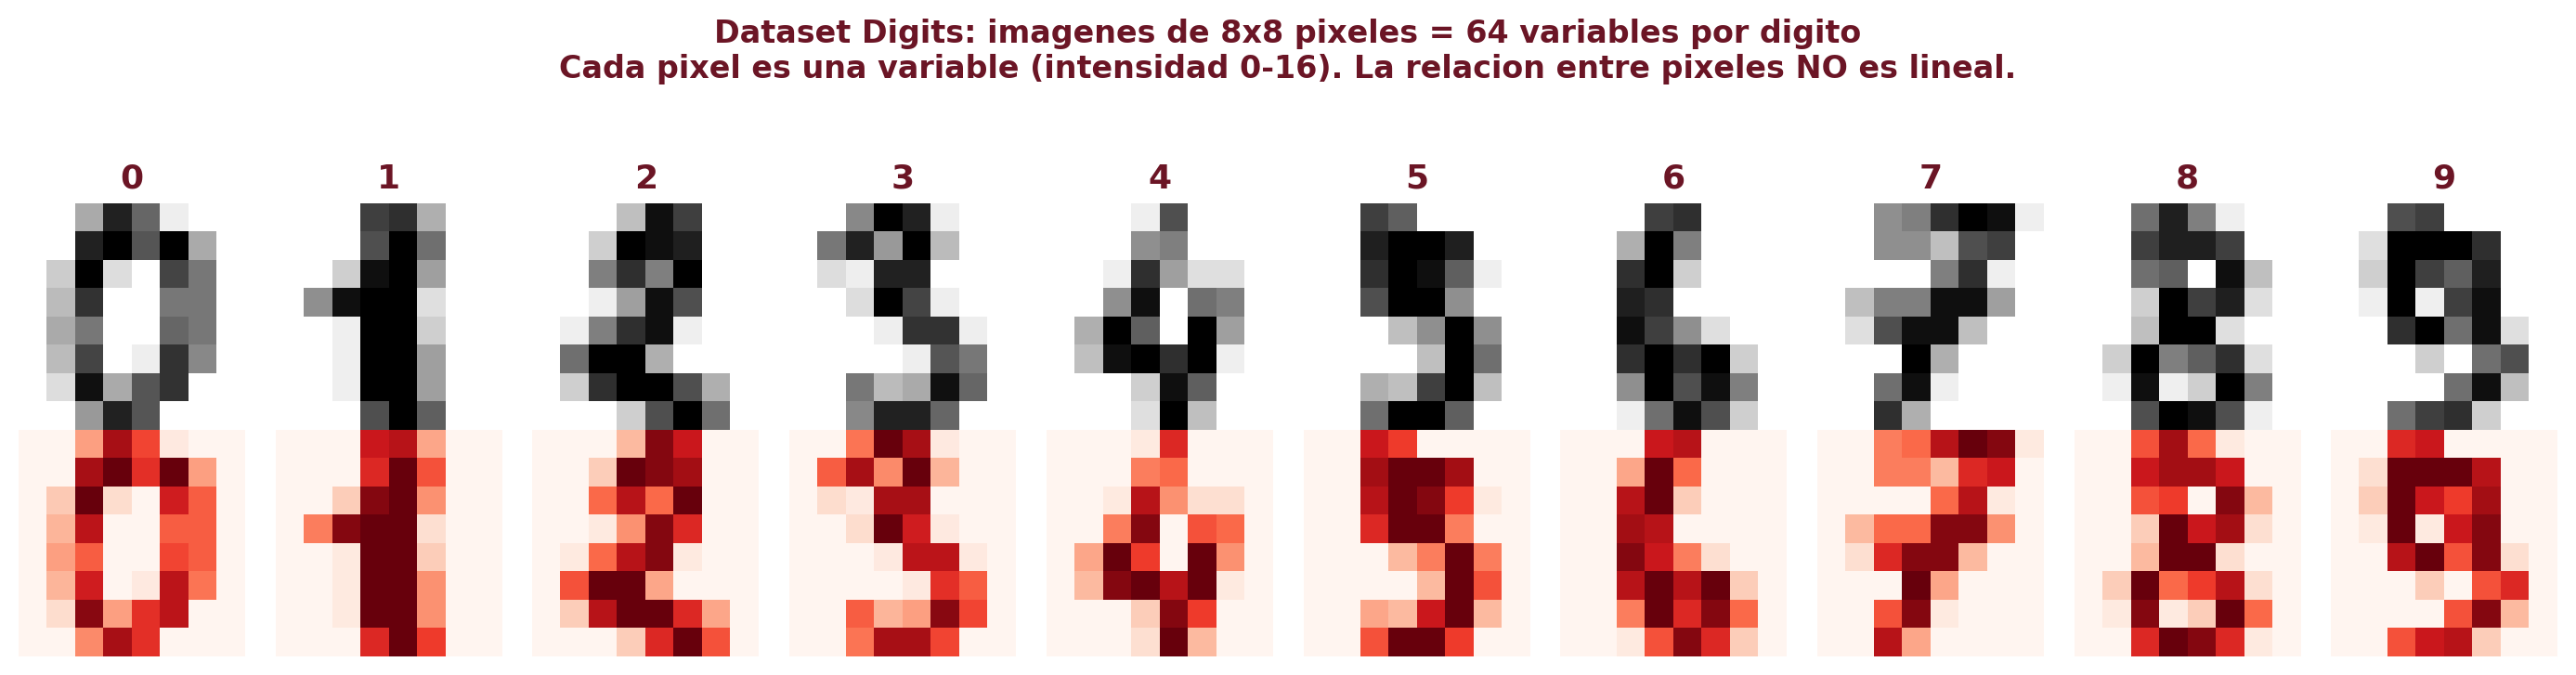
\includegraphics[width=0.9\textwidth]{fig_digits_ejemplos.png}
  \end{center}

  \vspace{-2pt}
  {\scriptsize\color{textMuted}
    \faLightbulb\hspace{4pt} Cada imagen es de $8 \times 8$ pixeles.
    Cada pixel tiene una intensidad de 0 (blanco) a 16 (negro).
    Esos 64 n\'umeros son las \textbf{64 variables} del dataset.
    Un ``5'' activa pixeles distintos que un ``0'' --- pero la relaci\'on
    entre pixeles es \textbf{compleja y no lineal}.}
\end{frame}

\begin{frame}[shrink=20]{?`Por Qu\'e las Im\'agenes No Son Lineales?}
  \vspace{-4pt}
  {\footnotesize\color{arcaDark}\bfseries
    La identidad de un d\'igito no est\'a en \textbf{un} pixel sino en la
    \textbf{forma} --- una relaci\'on geom\'etrica entre muchos pixeles.}

  \vspace{4pt}
  {\scriptsize
  \begin{itemize}\setlength{\itemsep}{3pt}
    \item[{\color{arcaRed}\scriptsize\faArrowRight}]
      Un ``0'' y un ``8'' pueden tener la \textbf{misma cantidad de tinta}
      (suma de pixeles parecida): un modelo lineal sobre la suma no los distingue.
    \item[{\color{arcaRed}\scriptsize\faArrowRight}]
      Mover el d\'igito 1 pixel a la derecha cambia \emph{todos} los valores
      de columna, pero es el \textbf{mismo n\'umero}: no hay relaci\'on
      lineal simple entre ``pixel (3,4) brillante'' y ``es un 8''.
    \item[{\color{arcaRed}\scriptsize\faArrowRight}]
      Lo que importa es \textbf{si hay un c\'irculo cerrado, una l\'inea recta,
      una curva en cierta zona} --- conceptos que requieren combinar pixeles
      de forma no lineal (curvas, bordes, esquinas).
  \end{itemize}
  }

  \vspace{4pt}
  \begin{center}
    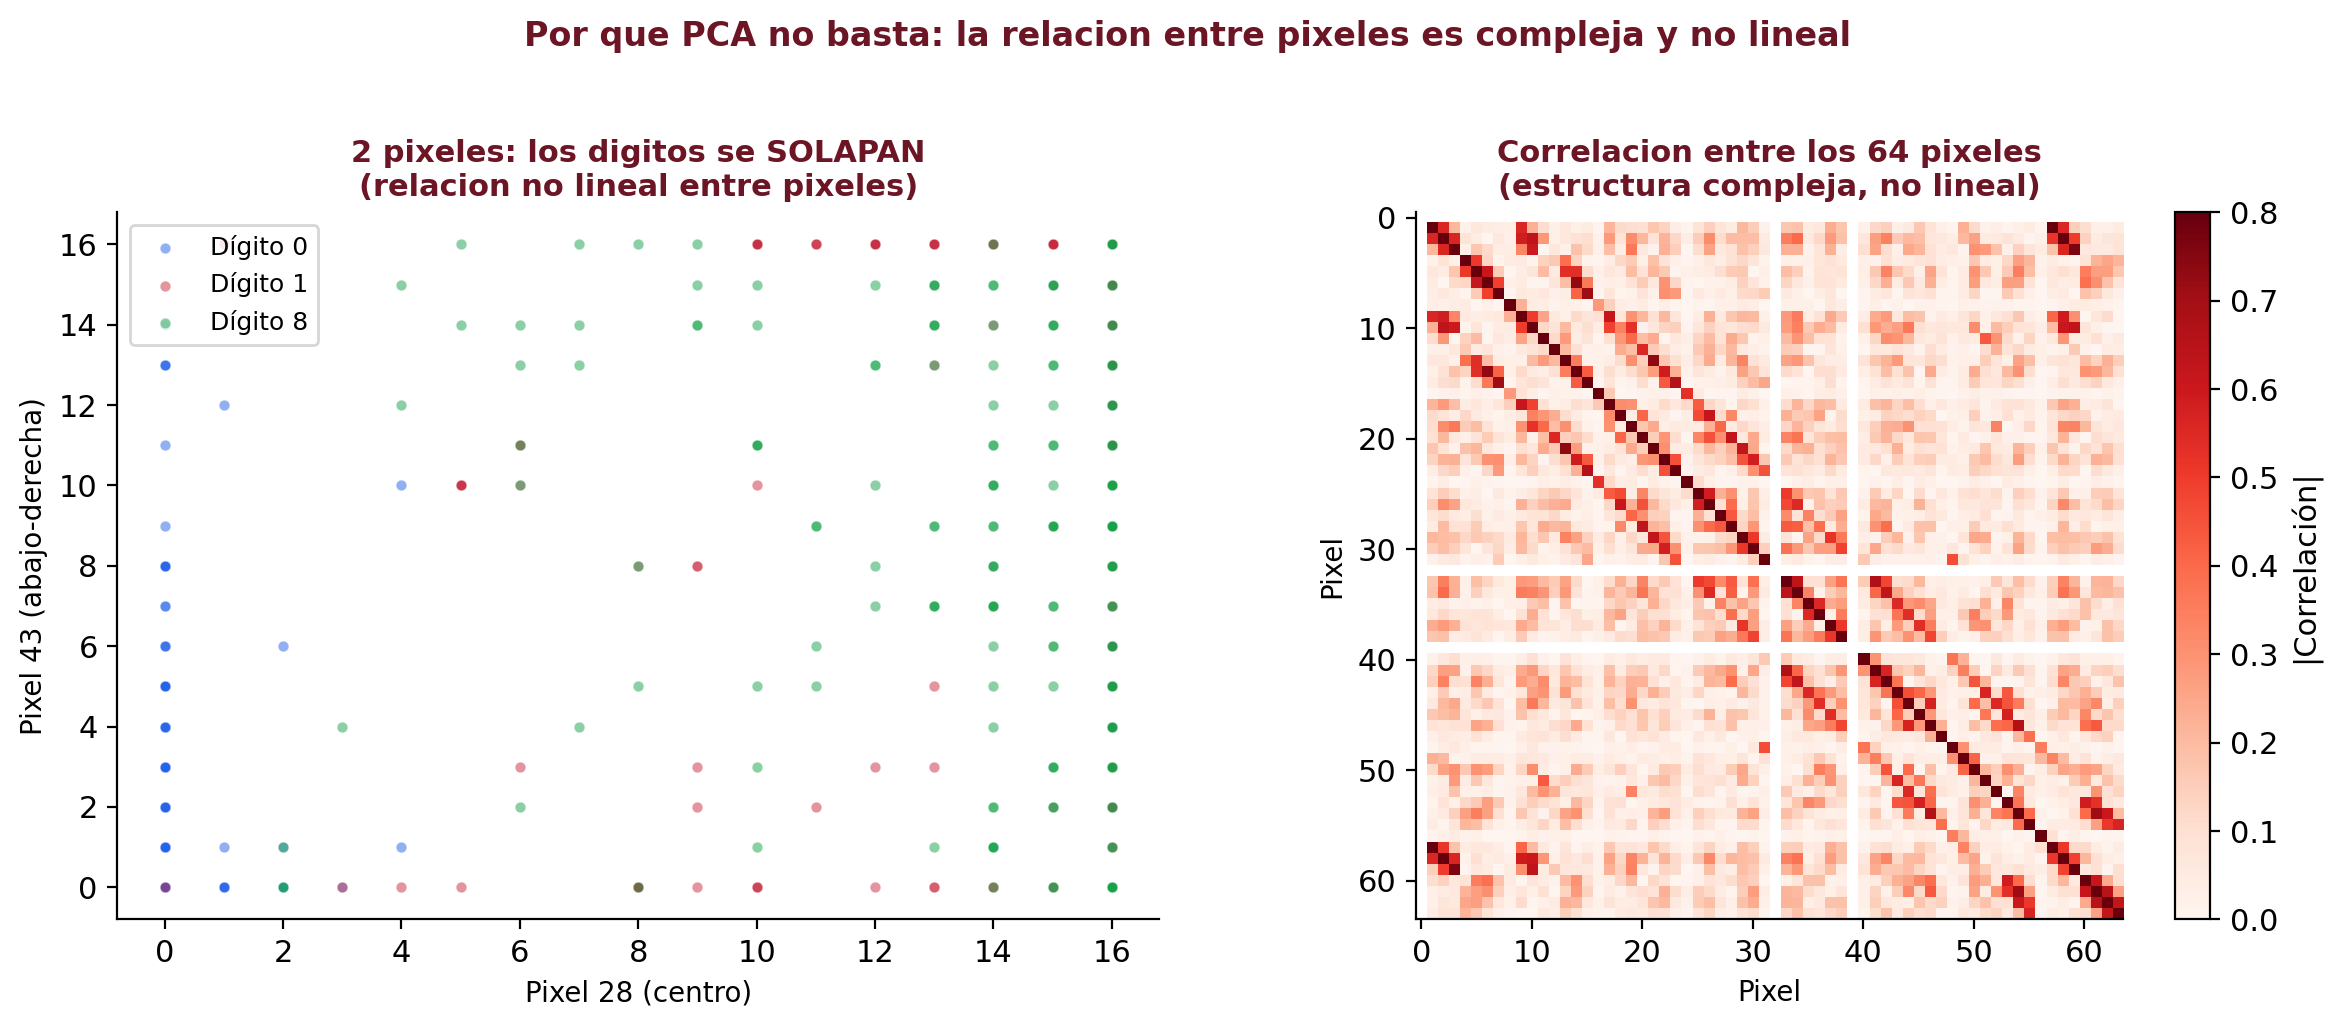
\includegraphics[width=0.78\textwidth]{fig_digits_nolineal.png}
  \end{center}

  \vspace{-2pt}
  {\scriptsize\color{textMuted}
    \faLightbulb\hspace{4pt} \textbf{Izquierda:} 2 pixeles cualesquiera no
    separan d\'igitos --- se solapan, ninguna recta los divide.
    \textbf{Derecha:} la matriz de correlaci\'on tiene bloques complejos,
    no la diagonal limpia que pedir\'ia un m\'etodo lineal.
    Por eso \textbf{PCA pierde estructura} y \textbf{t-SNE la captura}.}
\end{frame}

\begin{frame}[shrink=22]{PCA vs t-SNE en los D\'igitos}
  \vspace{-4pt}
  \begin{center}
    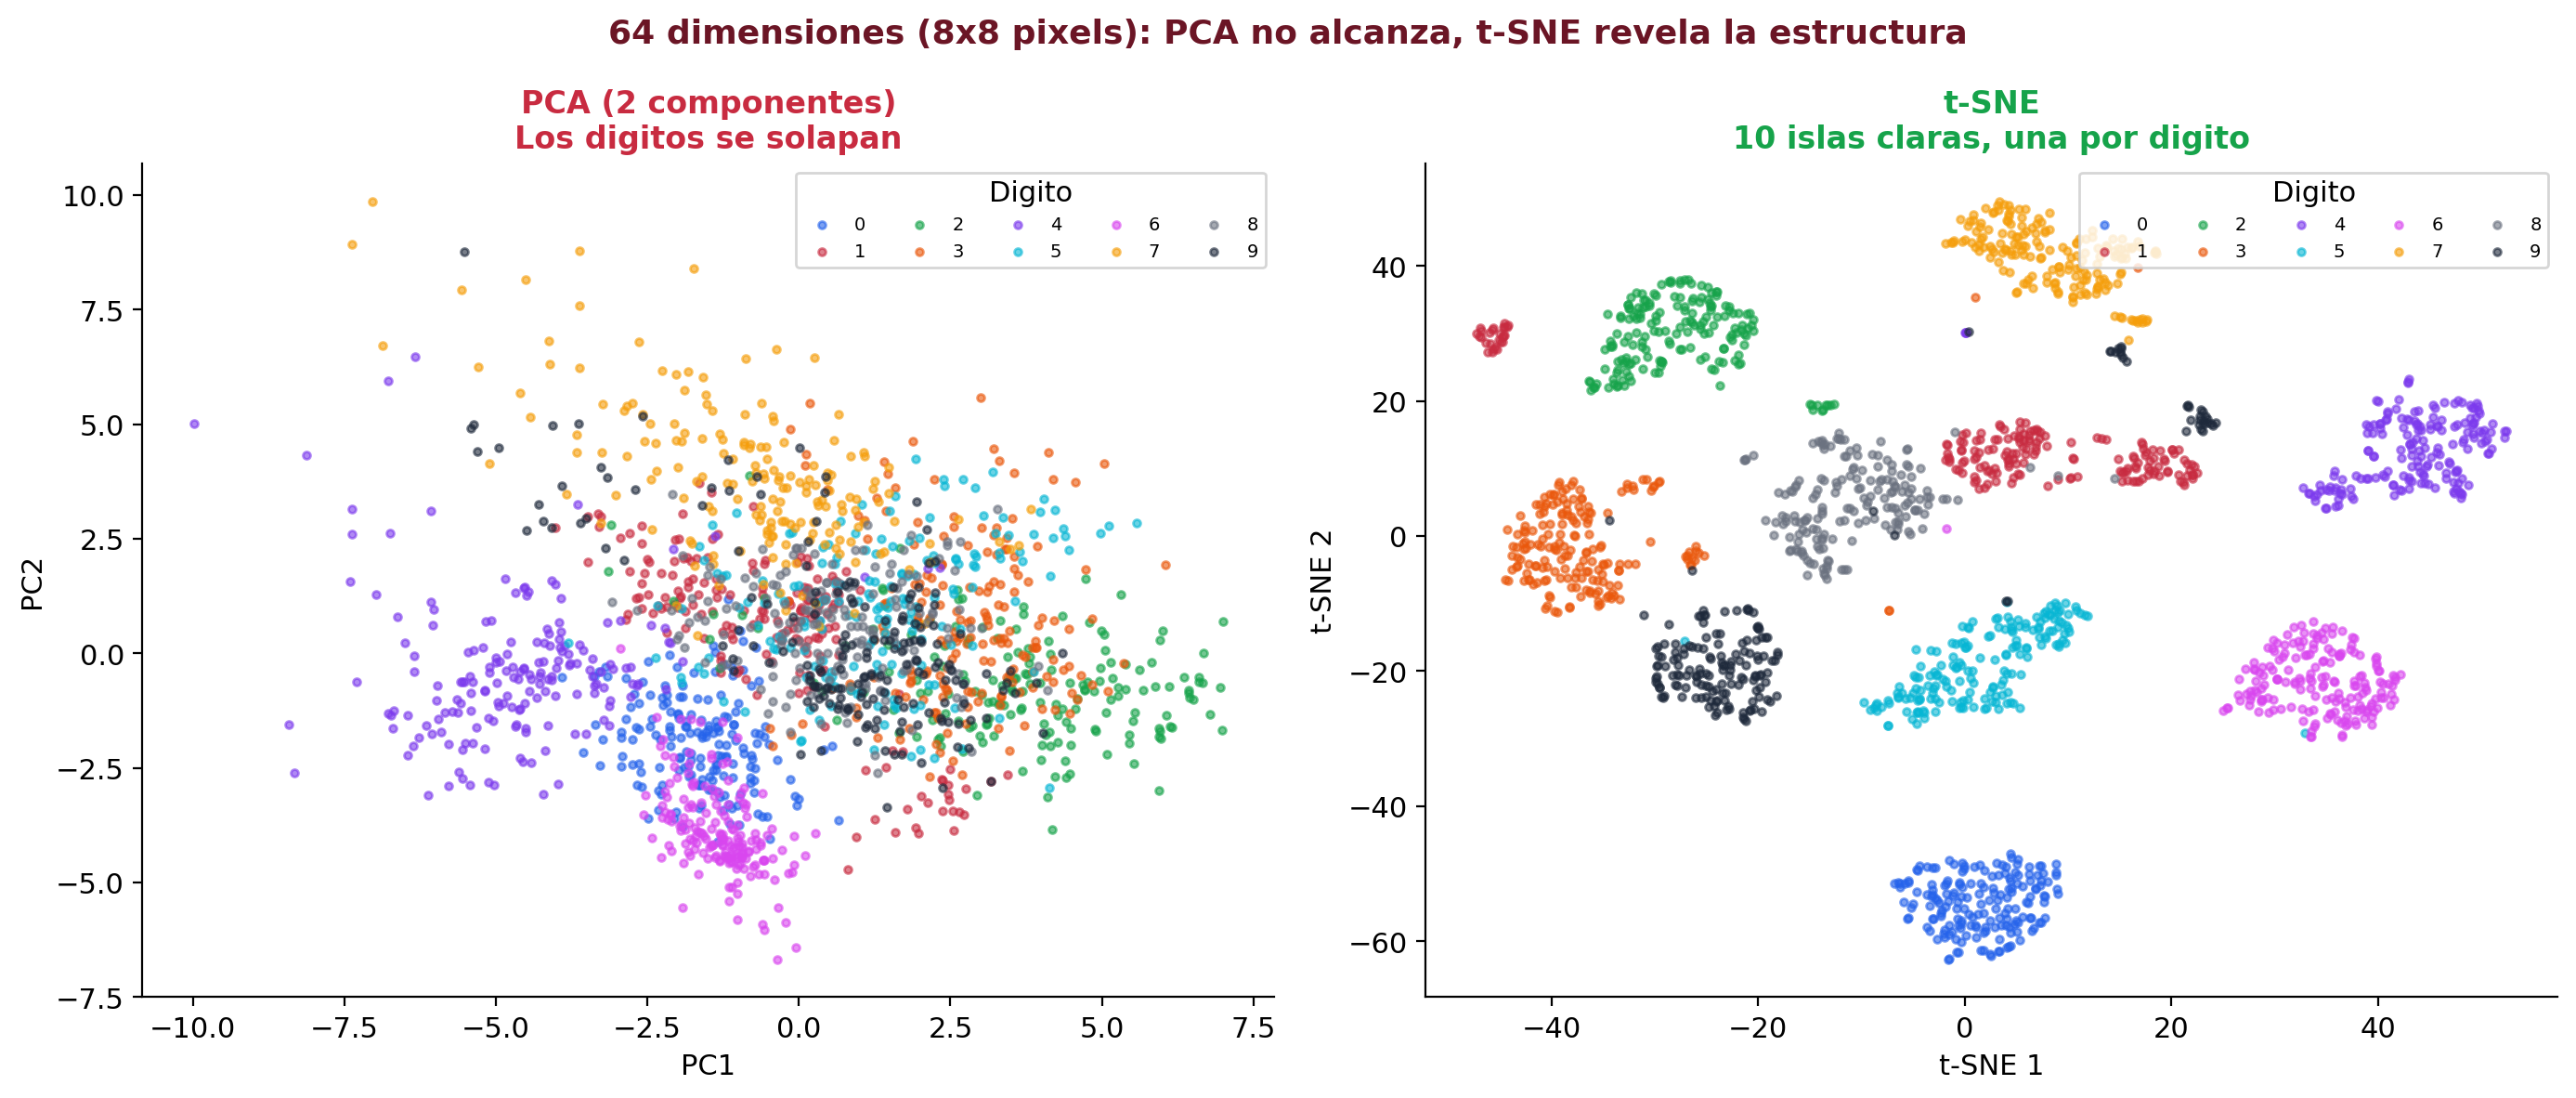
\includegraphics[width=0.92\textwidth]{fig_tsne_digits.png}
  \end{center}

  \vspace{-2pt}
  {\scriptsize\color{textMuted}
    \faLightbulb\hspace{4pt} 1797 im\'agenes de 8$\times$8 pixeles = 64
    dimensiones. \textbf{PCA (izquierda):} los d\'igitos se solapan,
    imposible distinguirlos. \textbf{t-SNE (derecha):} 10 islas claras,
    una por d\'igito. t-SNE captura la estructura no lineal que PCA pierde.}
\end{frame}

\begin{frame}[fragile,shrink=18]{C\'odigo: t-SNE en sklearn}
  \vspace{-6pt}
  \begin{pyblock}
from sklearn.manifold import TSNE
from sklearn.datasets import load_digits

digits = load_digits()   # 1797 imagenes, 64 pixeles
X_dig = digits.data

tsne = TSNE(n_components=2, random_state=42, perplexity=30)
X_tsne = tsne.fit_transform(X_dig)

# ATENCION: no tiene .transform() - no es parametrico
# tsne.transform(X_nuevo)  <-- ESTO NO EXISTE
  \end{pyblock}

  \vspace{4pt}
  {\scriptsize\color{arcaDark}
  \begin{itemize}\setlength{\itemsep}{3pt}
    \item[{\color{arcaRed}\scriptsize\faArrowRight}]
      \texttt{perplexity}: controla cu\'antos vecinos considera
      (t\'ipicamente 5--50). Probar varios valores.
    \item[{\color{arcaRed}\scriptsize\faArrowRight}]
      \textbf{No param\'etrico:} solo tiene \texttt{fit\_transform()},
      no \texttt{transform()}. No puede proyectar datos nuevos.
      Para eso, usar PCA.
    \item[{\color{codeGreen}\scriptsize\faArrowRight}]
      \textbf{Usar para:} visualizar. \textbf{No usar para:}
      preprocesamiento antes de K-Means (usar PCA).
  \end{itemize}
  }
\end{frame}

\begin{frame}{?`Cu\'ando Usar Cada Uno?}
  \vspace{-4pt}
  {\footnotesize\color{arcaDark}\bfseries
    Gu\'ia pr\'actica:}

  \vspace{6pt}
  {\footnotesize
  \begin{itemize}\setlength{\itemsep}{5pt}
    \item[{\color{codeBlue}\scriptsize\faArrowRight}]
      \textbf{PCA cuando:} quieres reducir dimensiones antes de un modelo
      (K-Means, RF), necesitas interpretar los componentes (loadings),
      tienes datos nuevos que proyectar, o pocas variables ($<$ 20).
    \item[{\color{codePurple}\scriptsize\faArrowRight}]
      \textbf{t-SNE cuando:} quieres \textbf{visualizar} datos de muy
      alta dimensi\'on (im\'agenes, texto, embeddings), no necesitas
      interpretar los ejes, y los datos tienen estructura no lineal.
    \item[{\color{codeGreen}\scriptsize\faArrowRight}]
      \textbf{Ambos:} PCA para reducir de 1000 a 50 dimensiones
      (quitar ruido), luego t-SNE para visualizar esas 50 en 2D.
      Es un pipeline com\'un en la pr\'actica.
  \end{itemize}
  }

  \vspace{4pt}
  \begin{tcolorbox}[colback=arcaGray, colframe=arcaRed, boxrule=0.5pt, arc=2pt,
    left=6pt, right=6pt, top=4pt, bottom=4pt]
    {\scriptsize\color{arcaDark}
    \faKey\hspace{4pt}\textbf{PCA = navaja suiza} (r\'apido, interpretable,
    param\'etrico). \textbf{t-SNE = microscopio} (revela detalles que PCA
    no ve, pero no sirve para todo lo dem\'as).}
  \end{tcolorbox}
\end{frame}

% =============================================================================
%  CIERRE
% =============================================================================
\sectionframe{Cierre}{Lo que aprendimos hoy}

\begin{frame}[shrink=10]{Resumen}
  \vspace{-4pt}
  \begin{columns}[T]
    \begin{column}{0.48\textwidth}
      {\footnotesize\bfseries\color{arcaDark} PCA:}
      \vspace{4pt}

      {\footnotesize
      \begin{itemize}\setlength{\itemsep}{3pt}
        \item[{\color{codeGreen}\faCheckCircle}]
          Comprimir muchas variables en pocas.
        \item[{\color{codeGreen}\faCheckCircle}]
          Scree plot: elegir cu\'antas conservar.
        \item[{\color{codeGreen}\faCheckCircle}]
          Loadings: interpretar qu\'e significa cada PC.
        \item[{\color{codeGreen}\faCheckCircle}]
          StandardScaler obligatorio.
      \end{itemize}
      }

      \vspace{4pt}
      {\footnotesize\bfseries\color{codeBlue} World Happiness:}
      \vspace{4pt}

      {\footnotesize
      \begin{itemize}\setlength{\itemsep}{3pt}
        \item[{\color{codeGreen}\faCheckCircle}]
          PC1 = desarrollo material (51.7\%).
        \item[{\color{codeGreen}\faCheckCircle}]
          PC2 = libertad y confianza (19.2\%).
        \item[{\color{codeGreen}\faCheckCircle}]
          3 clusters: desarrollados, transici\'on, en desarrollo.
      \end{itemize}
      }
    \end{column}

    \begin{column}{0.48\textwidth}
      {\footnotesize\bfseries\color{arcaRed} PCA + K-Means:}
      \vspace{4pt}

      {\footnotesize
      \begin{itemize}\setlength{\itemsep}{3pt}
        \item[{\color{codeGreen}\faCheckCircle}]
          PCA filtra ruido, K-Means segmenta.
        \item[{\color{codeGreen}\faCheckCircle}]
          Pipeline: scale $\to$ PCA $\to$ KMeans.
        \item[{\color{codeGreen}\faCheckCircle}]
          Clusters m\'as limpios que sin PCA.
      \end{itemize}
      }

      \vspace{4pt}
      {\footnotesize\bfseries\color{codePurple} t-SNE:}
      \vspace{4pt}

      {\footnotesize
      \begin{itemize}\setlength{\itemsep}{3pt}
        \item[{\color{codeGreen}\faCheckCircle}]
          No lineal: captura curvas y formas.
        \item[{\color{codeGreen}\faCheckCircle}]
          No param\'etrico: no tiene \texttt{.transform()}.
        \item[{\color{codeGreen}\faCheckCircle}]
          Para visualizar, no para preprocesar.
        \item[{\color{codeGreen}\faCheckCircle}]
          PCA + t-SNE: pipeline com\'un.
      \end{itemize}
      }
    \end{column}
  \end{columns}

  \vspace{6pt}
  \begin{tcolorbox}[colback=arcaRed!8, colframe=arcaRed, boxrule=0.5pt, arc=2pt,
    left=6pt, right=6pt, top=4pt, bottom=4pt]
    {\scriptsize\color{arcaDark}
    \faArrowRight\hspace{4pt}\textbf{Pr\'oxima clase:} Proyecto integrador
    --- aplicar todo lo aprendido a un problema real de principio a fin.}
  \end{tcolorbox}
\end{frame}

% ── QR ENCUESTA ──────────────────────────────────────────────────────────────
{
\setbeamertemplate{headline}{}
\setbeamertemplate{footline}{}
\begin{frame}[plain, noframenumbering]
  \begin{tikzpicture}[remember picture, overlay]
    \fill[arcaDark] (current page.south west) rectangle (current page.north east);
  \end{tikzpicture}
  \vspace{1cm}
  \begin{center}
    {\Huge\bfseries\color{white} ?`C\'omo estuvo la clase?\par}
    \vspace{0.6cm}
    
\includegraphics[width=4cm]{qr_encuesta.jpg}
    \vspace{0.4cm}

    {\large\color{white!80} Escanea el QR para dejarnos tu opini\'on.\par}
  \end{center}
\end{frame}
}

\end{document}
